% Options for packages loaded elsewhere
\PassOptionsToPackage{unicode}{hyperref}
\PassOptionsToPackage{hyphens}{url}
%
\documentclass[
  english,
]{article}
\title{Recruitment rate estimation in waterfowl using a non-invasive method}
\author{Adrien Tableau\footnote{Office Français de la Biodiversité, France - \href{mailto:adrien.tableau@ofb.gouv.fr}{\nolinkurl{adrien.tableau@ofb.gouv.fr}}} \and Iain Henderson\footnote{Animal and Plant Health Agency, United Kingdom - \href{mailto:iain.henderson@apha.gov.uk}{\nolinkurl{iain.henderson@apha.gov.uk}}} \and Sébastien Reeber\footnote{Société Nationale pour la Protection de la Nature, France - \href{mailto:sebastien.reeber@snpn.fr}{\nolinkurl{sebastien.reeber@snpn.fr}}}}
\date{15 décembre, 2021}

\usepackage{amsmath,amssymb}
\usepackage{lmodern}
\usepackage{iftex}
\ifPDFTeX
  \usepackage[T1]{fontenc}
  \usepackage[utf8]{inputenc}
  \usepackage{textcomp} % provide euro and other symbols
\else % if luatex or xetex
  \usepackage{unicode-math}
  \defaultfontfeatures{Scale=MatchLowercase}
  \defaultfontfeatures[\rmfamily]{Ligatures=TeX,Scale=1}
\fi
% Use upquote if available, for straight quotes in verbatim environments
\IfFileExists{upquote.sty}{\usepackage{upquote}}{}
\IfFileExists{microtype.sty}{% use microtype if available
  \usepackage[]{microtype}
  \UseMicrotypeSet[protrusion]{basicmath} % disable protrusion for tt fonts
}{}
\makeatletter
\@ifundefined{KOMAClassName}{% if non-KOMA class
  \IfFileExists{parskip.sty}{%
    \usepackage{parskip}
  }{% else
    \setlength{\parindent}{0pt}
    \setlength{\parskip}{6pt plus 2pt minus 1pt}}
}{% if KOMA class
  \KOMAoptions{parskip=half}}
\makeatother
\usepackage{xcolor}
\IfFileExists{xurl.sty}{\usepackage{xurl}}{} % add URL line breaks if available
\IfFileExists{bookmark.sty}{\usepackage{bookmark}}{\usepackage{hyperref}}
\hypersetup{
  pdftitle={Recruitment rate estimation in waterfowl using a non-invasive method},
  pdfauthor={Adrien Tableau; Iain Henderson; Sébastien Reeber},
  pdflang={en-EN},
  hidelinks,
  pdfcreator={LaTeX via pandoc}}
\urlstyle{same} % disable monospaced font for URLs
\usepackage[margin=1in]{geometry}
\usepackage{longtable,booktabs,array}
\usepackage{calc} % for calculating minipage widths
% Correct order of tables after \paragraph or \subparagraph
\usepackage{etoolbox}
\makeatletter
\patchcmd\longtable{\par}{\if@noskipsec\mbox{}\fi\par}{}{}
\makeatother
% Allow footnotes in longtable head/foot
\IfFileExists{footnotehyper.sty}{\usepackage{footnotehyper}}{\usepackage{footnote}}
\makesavenoteenv{longtable}
\usepackage{graphicx}
\makeatletter
\def\maxwidth{\ifdim\Gin@nat@width>\linewidth\linewidth\else\Gin@nat@width\fi}
\def\maxheight{\ifdim\Gin@nat@height>\textheight\textheight\else\Gin@nat@height\fi}
\makeatother
% Scale images if necessary, so that they will not overflow the page
% margins by default, and it is still possible to overwrite the defaults
% using explicit options in \includegraphics[width, height, ...]{}
\setkeys{Gin}{width=\maxwidth,height=\maxheight,keepaspectratio}
% Set default figure placement to htbp
\makeatletter
\def\fps@figure{htbp}
\makeatother
\setlength{\emergencystretch}{3em} % prevent overfull lines
\providecommand{\tightlist}{%
  \setlength{\itemsep}{0pt}\setlength{\parskip}{0pt}}
\setcounter{secnumdepth}{5}
\newlength{\cslhangindent}
\setlength{\cslhangindent}{1.5em}
\newlength{\csllabelwidth}
\setlength{\csllabelwidth}{3em}
\newlength{\cslentryspacingunit} % times entry-spacing
\setlength{\cslentryspacingunit}{\parskip}
\newenvironment{CSLReferences}[2] % #1 hanging-ident, #2 entry spacing
 {% don't indent paragraphs
  \setlength{\parindent}{0pt}
  % turn on hanging indent if param 1 is 1
  \ifodd #1
  \let\oldpar\par
  \def\par{\hangindent=\cslhangindent\oldpar}
  \fi
  % set entry spacing
  \setlength{\parskip}{#2\cslentryspacingunit}
 }%
 {}
\usepackage{calc}
\newcommand{\CSLBlock}[1]{#1\hfill\break}
\newcommand{\CSLLeftMargin}[1]{\parbox[t]{\csllabelwidth}{#1}}
\newcommand{\CSLRightInline}[1]{\parbox[t]{\linewidth - \csllabelwidth}{#1}\break}
\newcommand{\CSLIndent}[1]{\hspace{\cslhangindent}#1}
\usepackage{float}
\ifXeTeX
  % Load polyglossia as late as possible: uses bidi with RTL langages (e.g. Hebrew, Arabic)
  \usepackage{polyglossia}
  \setmainlanguage[]{english}
\else
  \usepackage[main=english]{babel}
% get rid of language-specific shorthands (see #6817):
\let\LanguageShortHands\languageshorthands
\def\languageshorthands#1{}
\fi
\ifLuaTeX
  \usepackage{selnolig}  % disable illegal ligatures
\fi

\begin{document}
\maketitle
\begin{abstract}
The response of a waterfowl population to a harvest pressure depends on its capacity to renew. The recruitment, i.e.~the number of young adults reproducing for the first time, is a key indicator to describe the renewal of a population, and therefore an essential tool in population management. The recruitment rate, defined inhere as the number of recruits produced per breeder, is even more informative because it is independent of the breeding population size and allows comparisons over time and between species. The proportion of young adult in a waterfowl population, which is a main step in estimating the recruitment rate, is often estimated from game-hunting samples. However, this proportion is not accessible in years without harvest, or with a low harvest rate. Moreover, the age-structure in the harvest samples does not necessarily reflect the underlying age-structure of the population. It is often skewed towards immatures and can lead to an overestimation of the recruitment rate. In waterfowl, adult males usually display brighter colours than females and immatures from both sexes. This dichromatism can be characterized and monitored from count surveys, a non-invasive method. Such information can be used to infer the proportion of immatures, and consequently the recruitment rate. In using two populations of ruddy duck, \emph{Oxyura oxyura}, this study introduces a model to estimate the recruitment rate from count data. To test the accuracy of the method, the results are compared to recruitment rate estimates from samples, and their consistency to support the observed population growth rates is also tested. The results suggest that the counting method is a versatile tool to estimate the recruitment rate if the species is monitored during the appropriate time window. Authors argue for considering a two-category count protocol in winter surveys of waterfowl species for which adult males can be differentiated from other individuals.

\textbf{Keywords}: fecundity - productivity - reproductive success - age ratio - juvenile - duck
\end{abstract}

\newpage

\hypertarget{introduction}{%
\section{Introduction}\label{introduction}}

\emph{Definitions}

One defines the recruitment rate of a breeding population as the average number of recruits produced per each breeder (\protect\hyperlink{ref-Flint2015}{Flint, 2015}). This parameter might sometimes be called \emph{annual fertility} (\protect\hyperlink{ref-Koons2014}{Koons et al., 2014}), \emph{fecundity} (\protect\hyperlink{ref-Arnold2018}{Arnold, 2018}), \emph{reproductive rate} (\protect\hyperlink{ref-Cooch2014}{Cooch et al., 2014}), \emph{reproductive success} (\protect\hyperlink{ref-Etterson2011}{Etterson et al., 2011}), or \emph{productivity} (\protect\hyperlink{ref-Hagen2008}{Hagen \& Loughin, 2008}; \protect\hyperlink{ref-Johnson1987}{D. H. Johnson et al., 1987}). If one considers a species reaching its sexual maturity as early as its first year, all individuals are mature at the reproduction season. The recruitment rate is thus the ratio of the number of young adults at the reproduction season of year \(t\), i.e.~the recruits, to the number of all individuals at the reproduction season of the previous year, \(t - 1\). The declination for species with delayed maturity follows the same process (see \protect\hyperlink{ref-Robertson2008}{Robertson, 2008}).

The recruitment rate parameter is complex because it is composed of two main sub-parameters: the fecundity followed by the juvenile survival (\protect\hyperlink{ref-Etterson2011}{Etterson et al., 2011}). Both sub-parameters can be split into other sub-parameters. The fecundity can be defined by the product of the nesting success, the average clutch size, and the hatching success. The juvenile survival can be defined as the product of the post-hatching survival and the post-fledging survival, both critical life periods (\protect\hyperlink{ref-Blums2004}{Blums \& Clark, 2004}; \protect\hyperlink{ref-Hill2008}{Hill \& Ellis, 2008}). The recruitment rate as defined in the present study is thus a parameter integrating multiple life steps from the egg to the young adult attempting to breed for its first time (\protect\hyperlink{ref-Koons2017}{Koons et al., 2017}).

\emph{The use of recruitment rate in population management}

Population conservation, harvesting, and control require tools in population management in order to reach quantitative targets, such as a population size for example (\protect\hyperlink{ref-Johnson2021}{F. A. Johnson et al., 2021}; \protect\hyperlink{ref-Shea1998}{Shea \& NCEAS Working Group on Population Management, 1998}). To do so, a first blind strategy is to test iteratively management rules to reach progressively an optimum. Such approach can be time-consuming given the intrinsic variability of the population response to its changing environment. It might also suffer from a rejection of the stakeholders because of the lack of transparency of an arbitrary process (\protect\hyperlink{ref-Williams2013}{Williams \& Madsen, 2013}). Another approach is to try to predict the growth rate of the population as a function of the harvest rate and other environment inputs. Such modelling approach can provide clues on the recovering time of a population upon a variety of management rules (\protect\hyperlink{ref-Otis2006}{Otis, 2006}). These decision-support tools are then key inputs to status on the best management rules to implement. The growth rate of a population depends on the adult survival and the recruitment rate, see Equation \eqref{eq:GR} in Section \ref{PGR}. The adult survival is generally estimated by mark recapture/recovery methods (\protect\hyperlink{ref-Lebreton2001}{Lebreton, 2001}). If the harvest pressure behaves as an additive mortality to the natural mortality for adults (e.g. \protect\hyperlink{ref-Iverson2013}{Iverson et al., 2013}), it is quite straightforward to predict its impact on the adult survival.

According to \protect\hyperlink{ref-Blums2004}{Blums \& Clark} (\protect\hyperlink{ref-Blums2004}{2004}), the recruitment for diving ducks is poorly related to fecundity, but depends mostly on juvenile survival, which is driven by weather conditions. Studies on other birds concludes also on the weak correlation between fecundity and recruitment (e.g. \protect\hyperlink{ref-Murray2000}{Murray, 2000}). The difficulty to track juvenile survival (\protect\hyperlink{ref-Schmidt2008}{Schmidt et al., 2008}) demonstrates the interest to focus on the recruitment rate when accessible. The key to predict the growth rate of a population is then to estimate the value of the recruitment rate and its variability, potentially influenced by the harvest pressure (\protect\hyperlink{ref-Anders2005}{Anders \& Marshall, 2005}).

\emph{The variability of the recruitment rate}

A waterfowl species that is released in a favourable habitat will naturally expand (\protect\hyperlink{ref-Malthus1872}{Malthus, 1872}). The growth of such a population reflects that the recruitment rate parameter is higher than the adult mortality rate. This expansion is limited by the carrying capacity of the habitat (\protect\hyperlink{ref-Sayre2008}{Sayre, 2008}). When a waterfowl species is endemic of an ecosystem and evolves in stable environmental conditions, the population size varies around the carrying capacity because the individuals compete for space or/and food (\protect\hyperlink{ref-Nummi2015}{Nummi et al., 2015}), which prevents the population from expanding. This competition commonly induces a lower fecundity or/and a higher juvenile mortality. The population renewal is slowed down because the recruitment rate parameter is affected by density-dependent effects (\protect\hyperlink{ref-Gunnarsson2013}{Gunnarsson et al., 2013}). For an endemic species evolving in stable environmental conditions, the recruitment rate compensates on average the adult mortality rate, which explains the stabilization of the number of individuals (\protect\hyperlink{ref-Flint2015}{Flint, 2015}).

Hunting waterfowl induces adult and juvenile mortality (\protect\hyperlink{ref-Bellrose1980}{Bellrose, 1980}). Intuitively, one expects that such a hunted population would observe lower adult survival and recruitment rate and then would rapidly deplete to its extinction. However, hunting waterfowl has a long history, and most of these species have persisted over time (\protect\hyperlink{ref-Cooch2014}{Cooch et al., 2014}). So paradoxically, hunting immature individuals does not always induce a decrease of recruitment rate. The heterogeneity of quality among immature individuals might explain this by inducing a compensation process if the harvest selects mostly individuals with a low reproductive potential (\protect\hyperlink{ref-Gimenez2017}{Gimenez et al., 2017}; \protect\hyperlink{ref-Lindberg2013}{Lindberg et al., 2013}). The recruitment rate can even increase because the harvest pressure reduces the densities and potentially the competition for space and food (\protect\hyperlink{ref-Nummi2015}{Nummi et al., 2015}; \protect\hyperlink{ref-Peron2012}{Péron et al., 2012}). In conclusion, a limited exploitation of a population observing heterogeneity and/or density-dependent process might paradoxically increase or at least not affect the recruitment rate. Under moderate exploitation, a new balance between recruitment rate and adult mortality can be theoretically reached (\protect\hyperlink{ref-Tsikliras2018}{Tsikliras \& Froese, 2018}). The size of a newly exploited population in stable environmental conditions should thus reach a different equilibrium, which is expected to be lower than the size without exploitation. This process explains why the exploitation of many waterfowl species is sustainable and has been lasting over a long time.

The fecundity and the juvenile survival, the two components of the recruitment rate, are very sensitive to weather conditions (\protect\hyperlink{ref-Blums2004}{Blums \& Clark, 2004}; \protect\hyperlink{ref-Folliot2017}{Folliot et al., 2017}). The environment conditions are thus an additional source of variability of the recruitment rate. The response of the recruitment rate to a harvest pressure is thus not straightforward. It is noisy because of its sensitivity to environmental factors. It also depends directly on the intensity of harvest on the immature individuals and indirectly on the mitigation of the density-dependent effects.

\emph{What part of the recruitment rate gradient is necessary for population management?}

In population management, a common question for a threaten or an invasive species is to determine the measure that will allow to reach a targeted population size/density in a limited time period (\protect\hyperlink{ref-Shea1998}{Shea \& NCEAS Working Group on Population Management, 1998}). For such question, the carrying capacity of the habitat is theoretically not reached. So a manager should mostly focus on collecting knowledge on the maximum recruitment rate and its variability by removing the potential density-dependent effects occurring only for the highest theoretical densities (\protect\hyperlink{ref-Eraud2021}{Eraud et al., 2021}; \protect\hyperlink{ref-Peron2013}{Péron, 2013}).

\emph{What is the ideal biological model to explore the gradient of the recruitment rate?}

Hunting waterfowl has a long history, but the biological effects of long-term moratorium have been poorly surveyed (\protect\hyperlink{ref-MartinezAbrain2013}{Martínez-Abraín et al., 2013}). So there are few opportunities to explore the response of the recruitment rate to a gradient of pressure for such species. Alien vertebrate species are commonly introduced during release events (\protect\hyperlink{ref-Saul2016}{Saul et al., 2016}). They usually observe a first period of colonisation on new territories without management measures. Since its presence might impact the balance of the colonized ecosystem, it happens that managers take strong control measures to restrict the growth of these populations or to eradicate them (\protect\hyperlink{ref-Oficialdegui2020}{Oficialdegui et al., 2020}). Such species are then a good biological model to overcome density-dependent effects and explore the effects of a harvest gradient on recruitment rate.

\emph{How to estimate recruitment rate?}

The recruitment rate parameter of a population can be assessed first by evaluating the fecundity of the breeding population and then by monitoring the survival from the egg life stage to the first-breeding event. To do so, it is necessary to monitor nests in habitats representative of the considered population (\protect\hyperlink{ref-Blums2004}{Blums \& Clark, 2004}). The survival of a chick to its recruitment can be done by capture mark recapture method quite tricky to set up (\protect\hyperlink{ref-Arnold2018}{Arnold, 2018}; \protect\hyperlink{ref-Blums2004}{Blums \& Clark, 2004}; \protect\hyperlink{ref-Schmidt2008}{Schmidt et al., 2008}). Even if such approach provides valuable information on the dynamics of the recruitment and can highlight the bottlenecks, the fieldwork required to estimate both components is too time-consuming to generalize such approach for waterfowl population management on a long-term horizon.

In waterfowl, it is generally impossible to differentiate immatures from adults without examining birds in hand. Aging individuals from samples coming from hunting bags is thus another opportunity to estimate the recruit proportion. Such approach suffers from two caveats. First, it is impossible to assess the recruitment rate when there is no harvest whereas it is necessary to predict what would happen if a moratorium seems required to allow a population to recover, or to calibrate a priori the harvest effort necessary to control an invasive species (\protect\hyperlink{ref-Smith2005}{G. C. Smith et al., 2005}). Secondly, like any predation action, hunting is selective and provides a biased picture of the population age structure in favour of the immatures (\protect\hyperlink{ref-Bellrose1980}{Bellrose, 1980}; \protect\hyperlink{ref-Fox2014}{A. D. Fox et al., 2014}). The hunting bag analysis might then lead to overestimate the recruitment rate and consequently the maximum sustainable harvest rate, with adverse consequences on population conservation (\protect\hyperlink{ref-Fox2014}{A. D. Fox et al., 2014}). Inferring recruitment rate from the proportion of immature birds trapped during tagging studies is also promising (\protect\hyperlink{ref-Arnold2018}{Arnold, 2018}), but the author admits that juveniles might be more naïve and are then more likely caught in traps (\protect\hyperlink{ref-RguibiIdrissi2003}{Rguibi-Idrissi et al., 2003}).

In waterfowl, it is common that adult males display brighter colours than adult females and immatures of both sexes, which display cover-up plumage similar to adult females (\protect\hyperlink{ref-Johnson1999}{K. P. Johnson, 1999}). This discrepancy is valuable because it can be observed and quantified from distance. Knowing adult sex ratio, such approach is promising because it requires only to count the proportion of birds of the two plumage kinds to infer the recruitment rate (\protect\hyperlink{ref-Smith2001}{C. M. Smith et al., 2001}). Unlike the two previous methods, this one is non-invasive and requires an acceptable time investment, which allows to collect long time series and consequently to track recruitment rate variability.

\emph{Methodology of this study}

From two populations of ruddy duck, a species introduced in Europe in the 40's, this study introduces a simple Bayesian model to infer recruitment rate from count data. A large part of this study focuses on assessing the viability of such approach. The comparison between two populations is a first step in testing the consistency of the method. A comparison to the common approach using samples from hunting bags aims at checking if the recruitment rate variability is well tracked and if the hypothesis stating that the recruitment rate is overestimated when using sample data is consistent with the results. Using two other approaches using population growth rates, one testes the consistency of the order of magnitude of the recruitment rate estimated from the counting method. Studying two populations is also an opportunity to discuss the response of the recruitment rate to a gradient of harvest pressure.

\hypertarget{MM}{%
\section{Materials \& methods}\label{MM}}

\hypertarget{biological-model}{%
\subsection{Biological model}\label{biological-model}}

The ruddy duck is a diving duck species introduced in the United Kingdom in the 40's (\protect\hyperlink{ref-GutierrezExposito2020}{Gutiérrez-Expósito et al., 2020}). The first reproduction was observed in the 60's. The population rapidly grew to reach more than 5000 individuals spread over the entire country. A new population set up in France from the 90's, likely because of an arrival of a few individuals from the United Kingdom (UK). Unlike the UK population, the French one set up around a single wintering spot, the Grand Lieu Lake (47.09°N, 1.67°W), which facilitates the population monitoring. Since this species is considered as a threat to the white-headed duck because of the risk of a genetic introgression (\protect\hyperlink{ref-MunozFuentes2007}{Muñoz-Fuentes et al., 2007}), an European plan of eradication has been adopted and control measures were taken in both countries (\protect\hyperlink{ref-GutierrezExposito2020}{Gutiérrez-Expósito et al., 2020}).

Just before the reproduction period, one can distinguish from shore individuals with male-like plumage from female-like individuals on wintering spots (Figure \ref{fig:flock}). It is noticeable that the apparent proportion of males in the counts from shore is far below the proportion of males in the samples from hunting bags (Figure \ref{fig:pmal}).

\begin{figure}[H]

{\centering 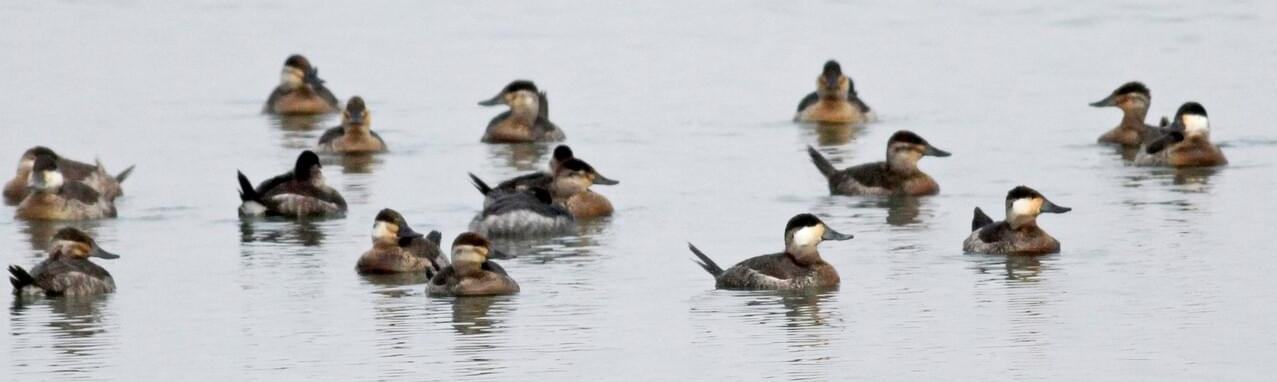
\includegraphics[width=1\linewidth]{../Output/flock} 

}

\caption{Typical observation of a ruddy duck flock in winter: 4 male-like individuals with a white cheek and a black cap, 10 female-like individuals with a whitish cheek and a dark stripe across it, 3 unidentified individuals © Jay McGowan - 3 February 2013 - Tompkins, New York, United States}\label{fig:flock}
\end{figure}

\begin{figure}[H]

{\centering 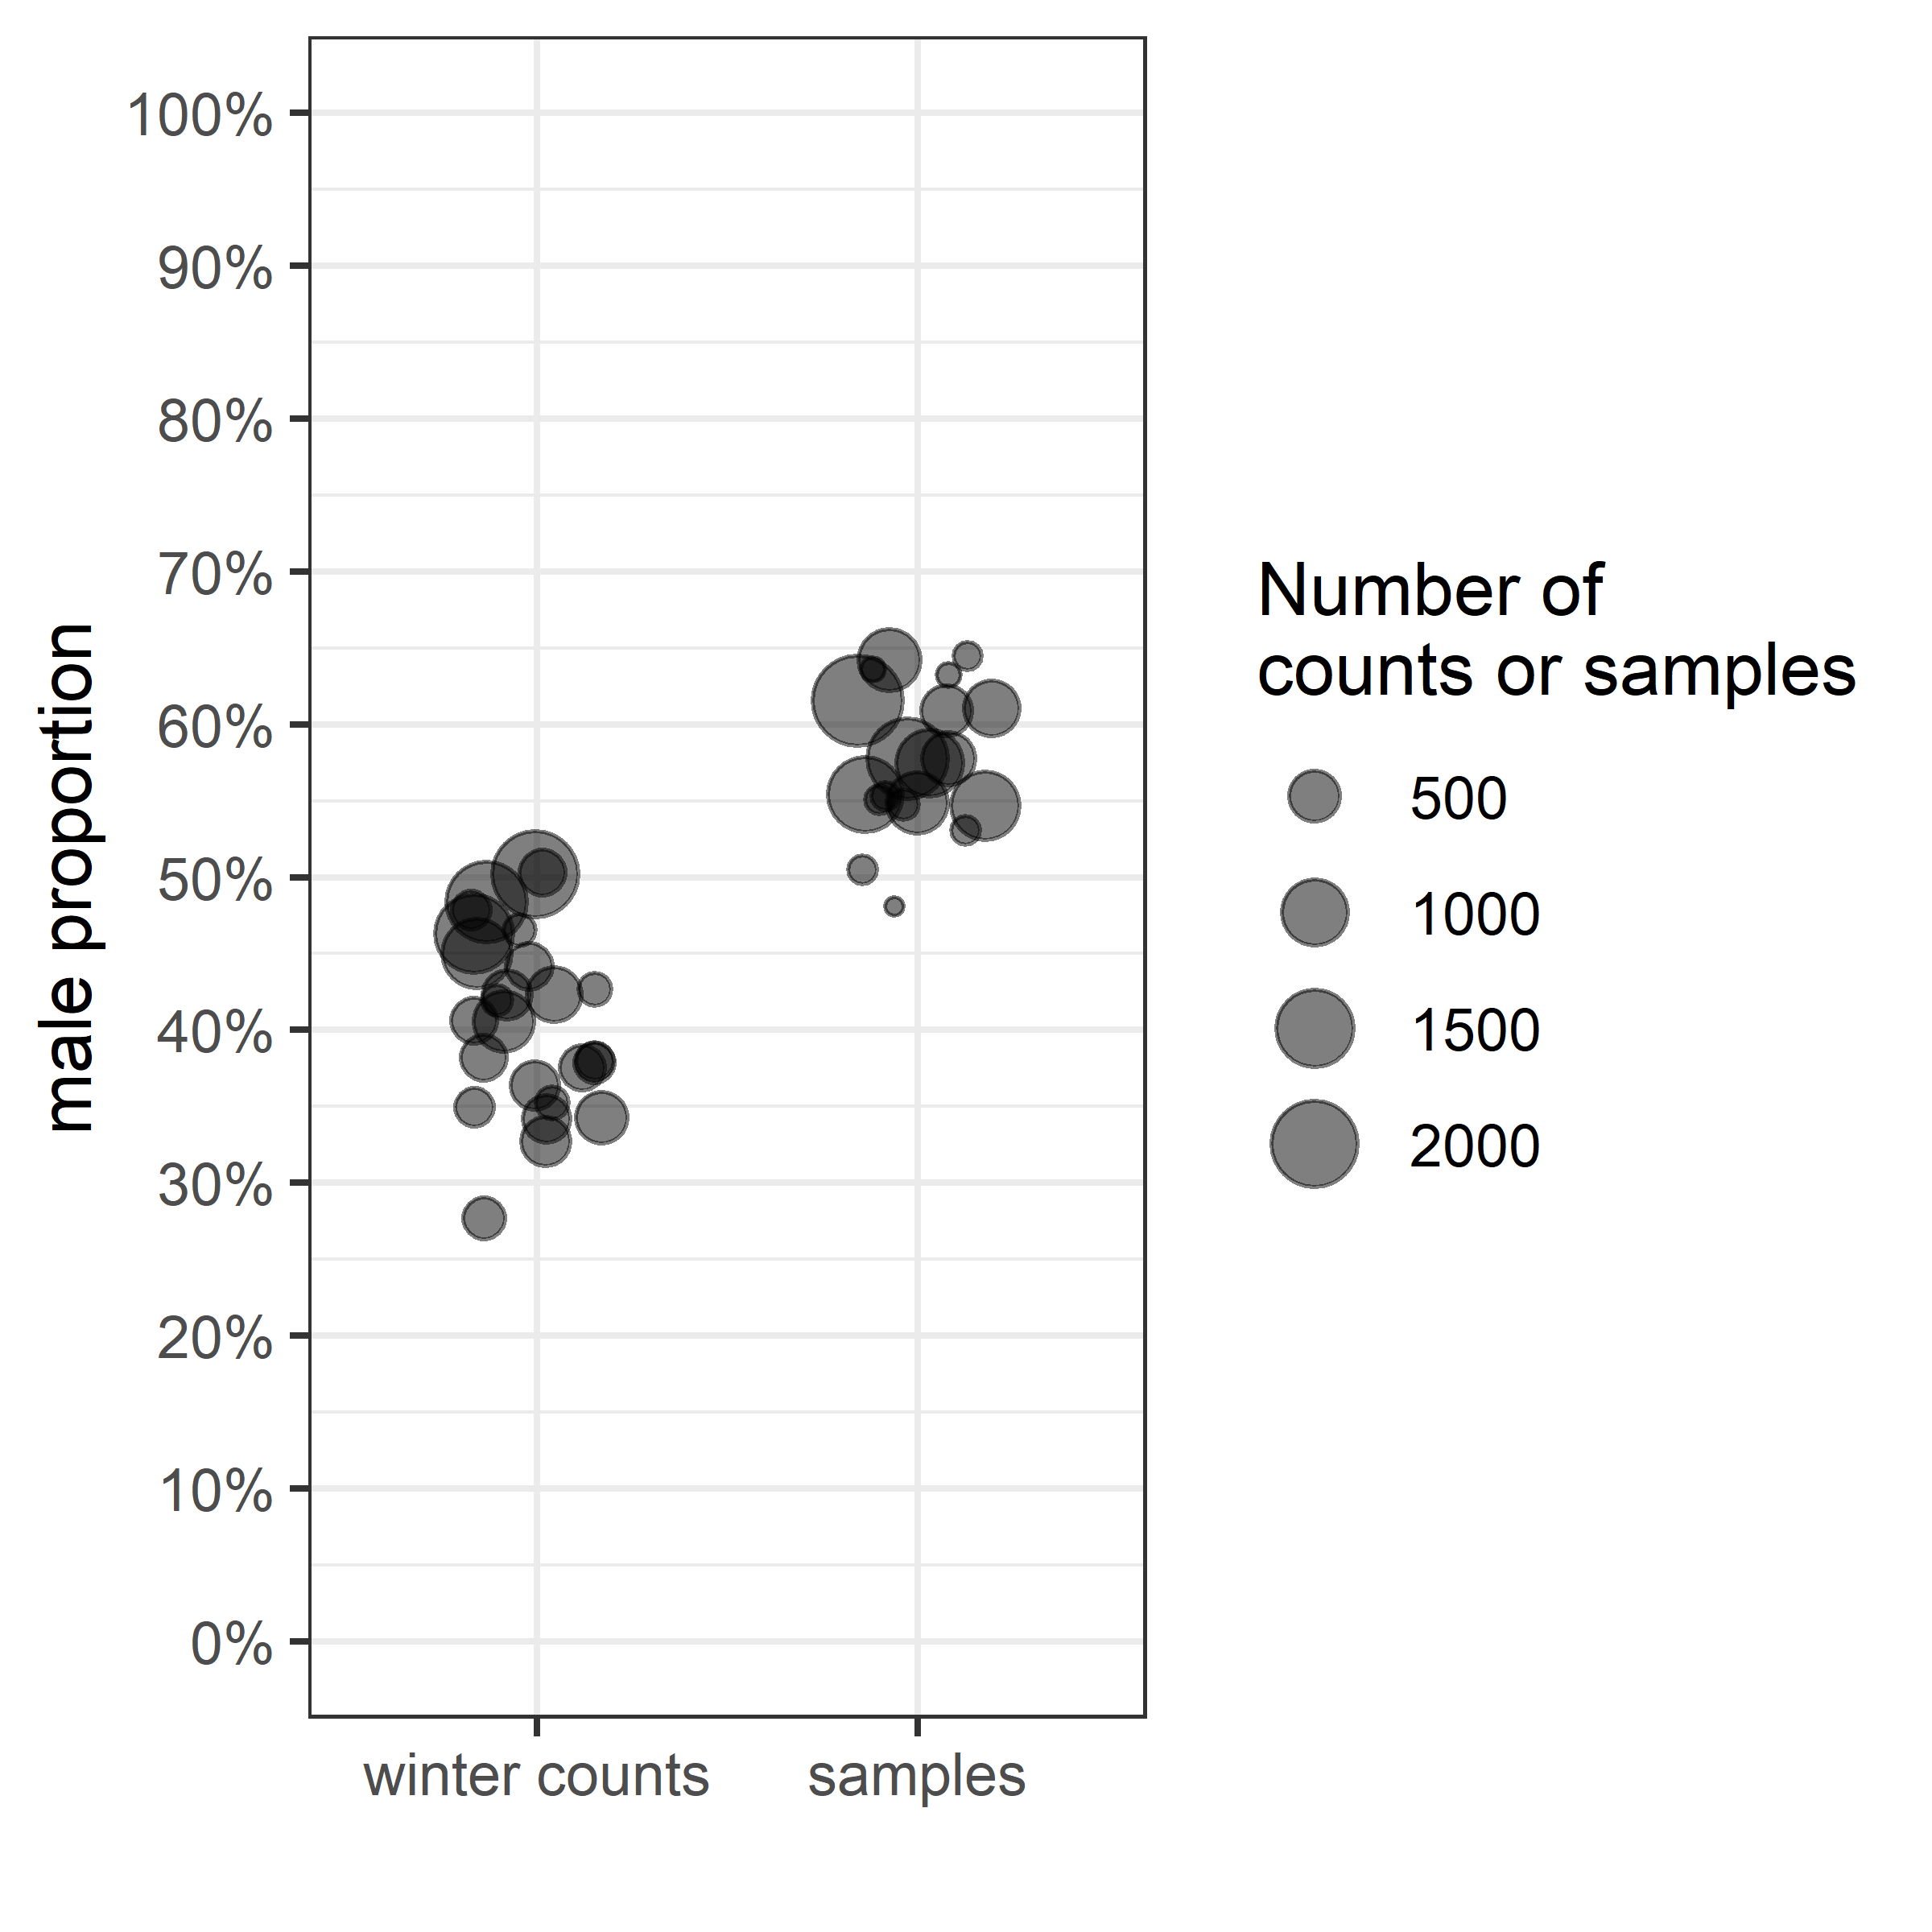
\includegraphics[width=1\linewidth]{../Output/plot_1_saved} 

}

\caption{Apparent male proportion in winter counts vs male proportion in samples; for the first category, one point corresponds to the proportion of male-like plumage in a population counted in winter; for the second category, the male proportion is estimated from all ruddy ducks sampled over one year}\label{fig:pmal}
\end{figure}

Assuming sex identification of samples is very accurate, such observation demonstrates that the counting method misses the identification of a significant part of males in the population. In many waterfowl species, immature individuals of both sexes display cover-up plumage similar to adult females (\protect\hyperlink{ref-Reeber2015}{Reeber, 2015}). Consequently, the counts in winter allows adult males to be distinguished from all other individuals (adult females, immature females, and immature males). This feature can be valuable to estimate the recruitment with two conditions. The season when adult males can be distinguished from all other individuals is sufficiently close to the breeding period to consider the age structure picture of the population to be representative of the age structure of the breeding population. The adult sex ratio is known and stable over the considered time period.

The demography of both ruddy duck populations has been tracked thanks to exhaustive counts on the wintering spots during the period between December 1 and January 31. Controlled individuals between the counting date and the beginning of the reproduction period (set up to May 1 upon field observations) were subtracted from the winter count to get a proxy of the breeding population size. Time series show that the two populations follow similar demographic histories (Figure \ref{fig:count}). They grew freely in both countries until 1999. Control measures have been then applied from 1999 to 2005 in the UK and from 1999 to 2018 in France. In both countries, these management measures led to stop the expansion of the ruddy ducks. From 2005 in the UK and from 2018 in France, higher control effort led to a rapid depletion in both populations. This history underlines that both populations observed a large spectrum of harvest effort, from no pressure to very high pressure. For sake of interpretation, the time period 2001-2004 was classified in the \emph{no harvest} category in France because the harvest pressure applied over this period was very limited with no effect on the population growth.

\begin{figure}[H]

{\centering 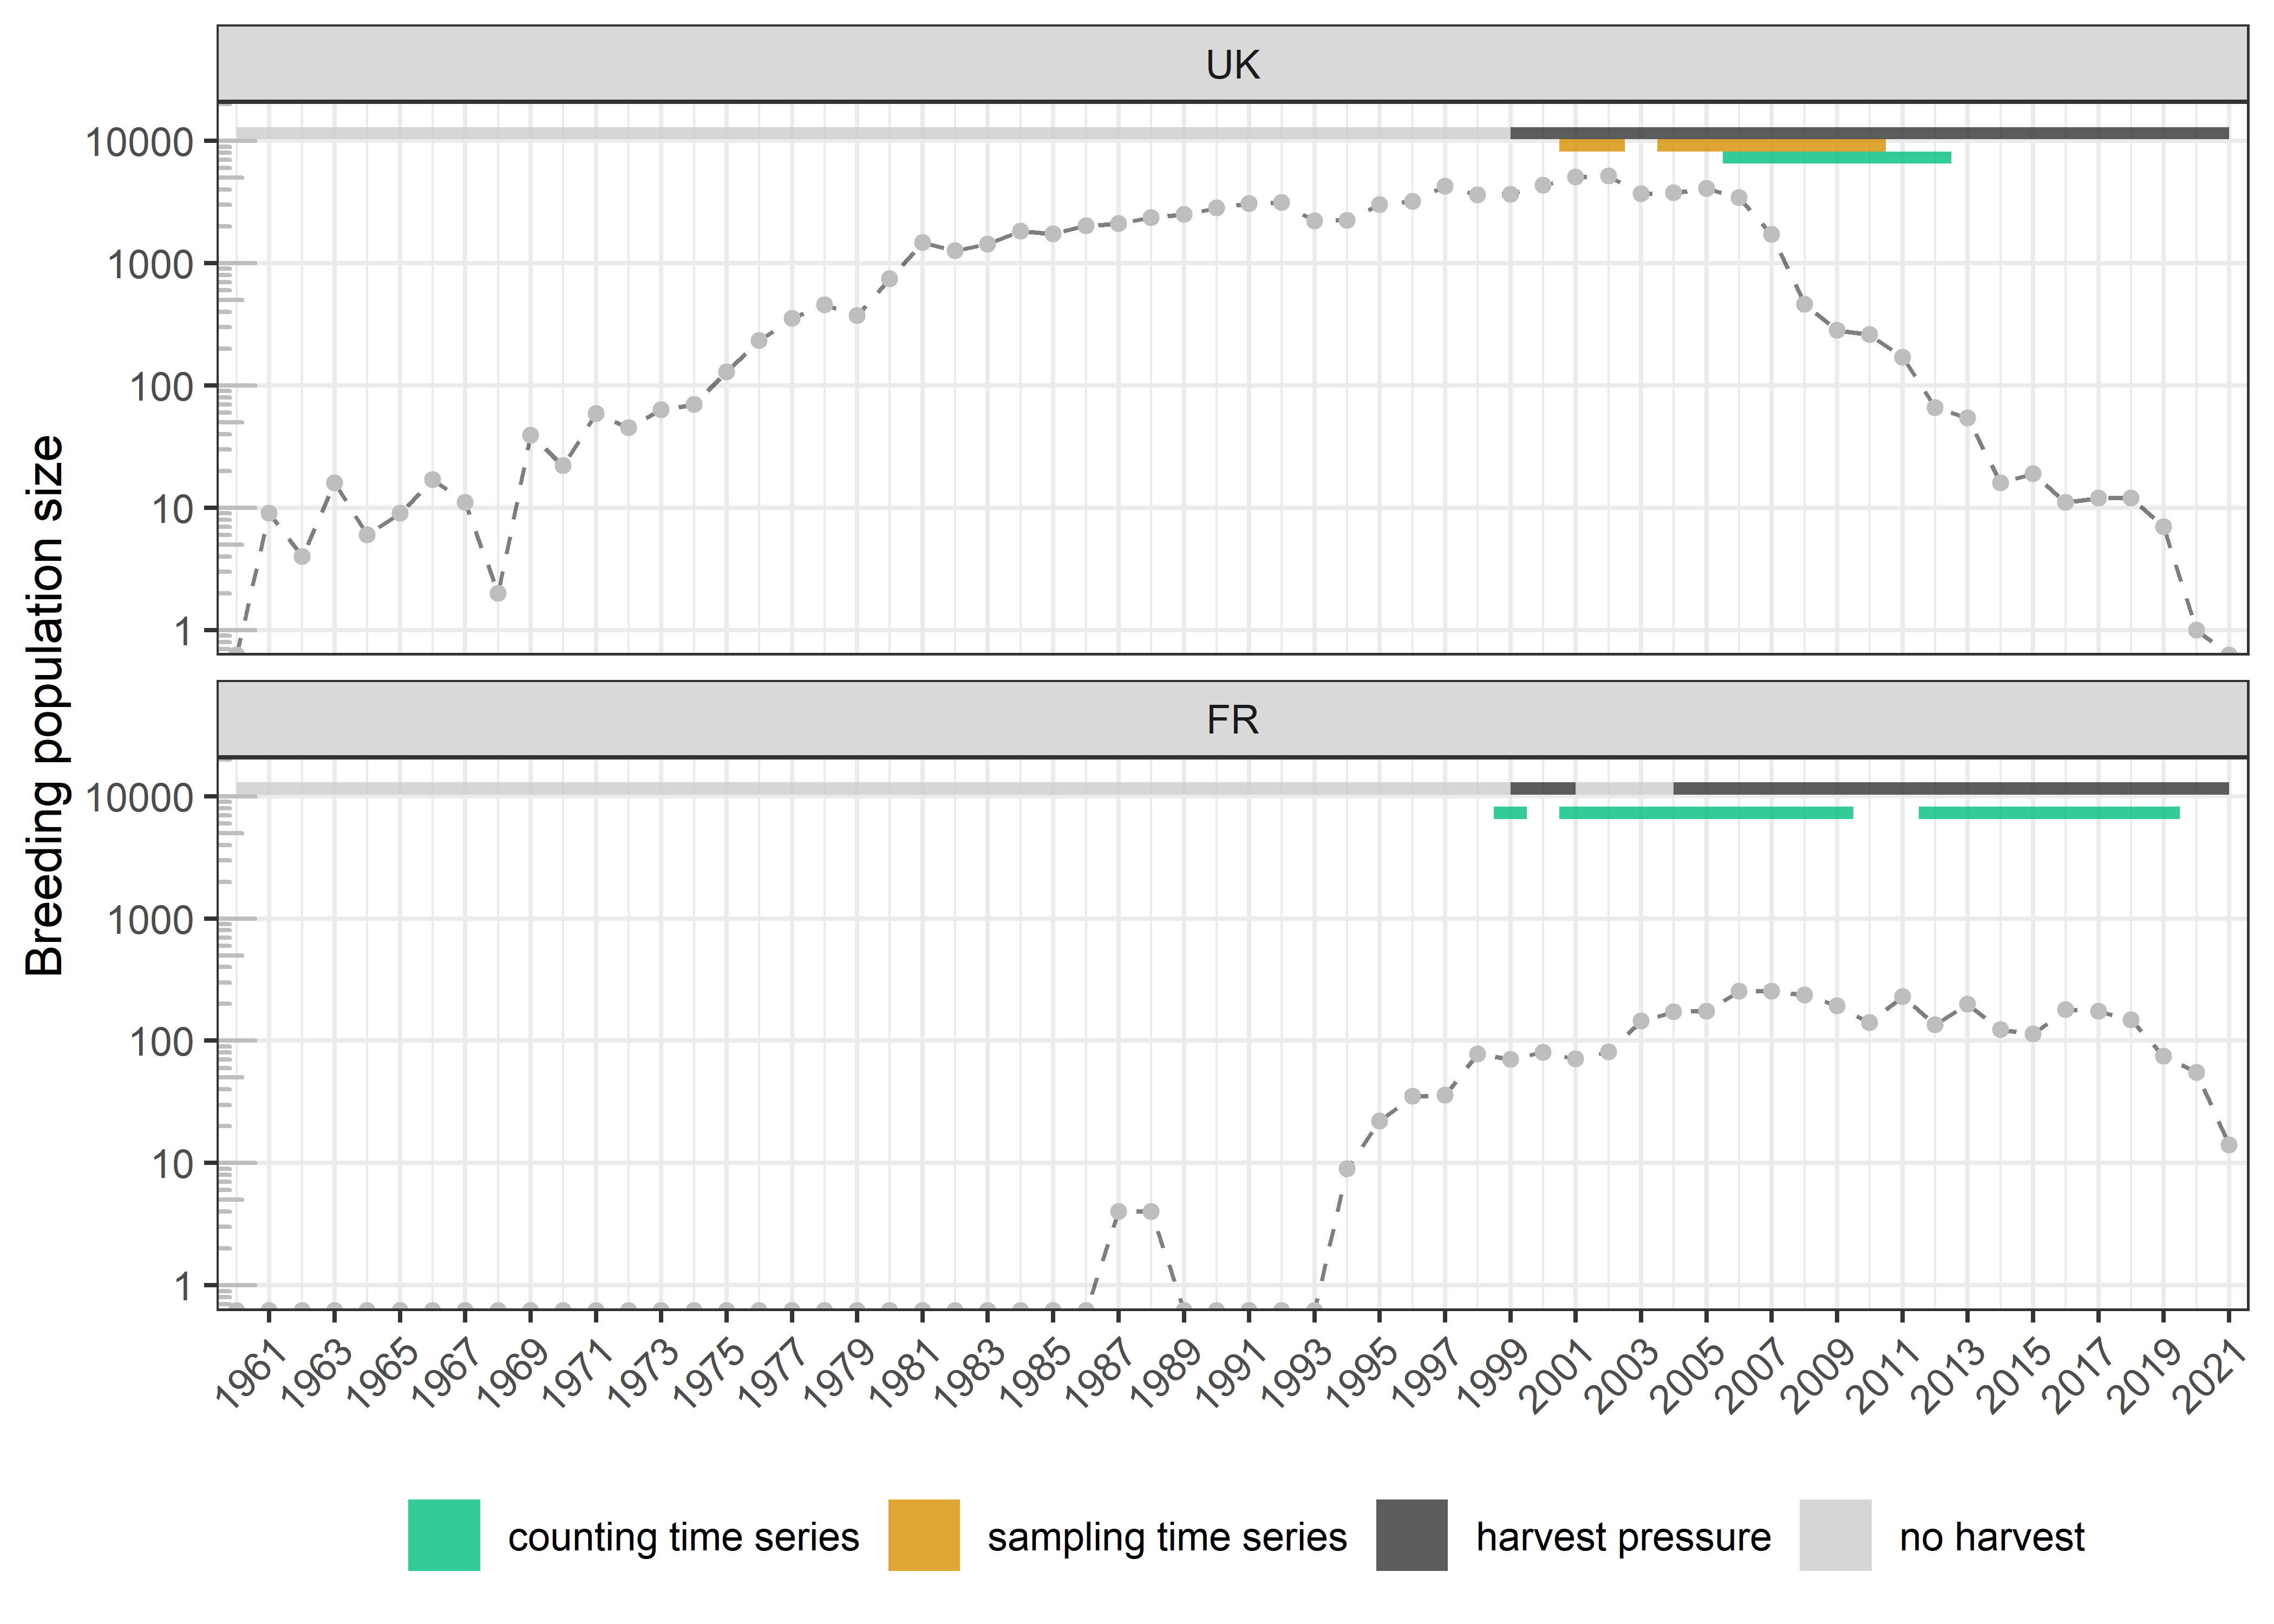
\includegraphics[width=1\linewidth]{../Output/plot_2} 

}

\caption{Evolution of the size of the two ruddy duck populations in light of the harvest pressure and the data time series}\label{fig:count}
\end{figure}

The counting dataset, which differentiates the male-like from the female-like individuals in winter, covers 7 years and 19 years in UK and France respectively (Figure \ref{fig:count}). Combined together, the counting datasets cover different population dynamics corresponding to a gradient of harvest pressure. In France, data before 2004 correspond to a period of population growth with (almost) no harvest pressure, whereas data in the following years correspond to a stabilized population size with a significant level of harvest pressure (Figure \ref{fig:count}). In UK, the counting data correspond to a quick population depletion associated to a high level of harvest pressure, especially before the reproduction period. In parallel, the sampling dataset, which corresponds to individuals shot in winter during control operations, covers 9 years only in UK, with 5 years in common with the corresponding counting time series.

\hypertarget{recruitment-rate-inference-from-count-data}{%
\subsection{Recruitment rate inference from count data}\label{recruitment-rate-inference-from-count-data}}

Adult sex ratio in waterfowl is generally biased towards males (Figure \ref{fig:pmal}, \protect\hyperlink{ref-Wood2021}{Wood et al.} (\protect\hyperlink{ref-Wood2021}{2021})). As a consequence, deducing the immature proportion from the adult male proportion is not straightforward because the adult proportion twice as much as the male proportion. Even if the adult sex ratio may vary over a long time range, it is relatively stable over a few years (\protect\hyperlink{ref-Wood2021}{Wood et al., 2021}). Sex identification in adult samples from hunting bags was available for both ruddy duck populations. However, the small population size in France prevents from providing precise sex proportion estimates. A comparison over months in UK showed no difference in male proportion, so adult samples collected over the whole year were used to estimate the male proportion. A comparison of male proportion among years with more 500 samples did not show significant interannual differences. As a consequence, all adult samples were pooled to estimate the adult male proportion, see Equation \eqref{eq:pm}.

Assuming the additive property of the binomial distribution, the proportion of immature individuals can be deduced from the cumulated counts of male-like individuals in the wintering population, see Equation \eqref{eq:pic}. Only years with more than 100 individuals were selected. From this proportion and abundance index of breeding population sizes, the recruitment rate is straightforward, see Equation \eqref{eq:r}. If the absolute value of the breeding population size is accessible, the recruitment can be estimated, see Equation \eqref{eq:R}.

\begin{longtable}[]{@{}
  >{\raggedright\arraybackslash}p{(\columnwidth - 4\tabcolsep) * \real{0.11}}
  >{\raggedright\arraybackslash}p{(\columnwidth - 4\tabcolsep) * \real{0.13}}
  >{\raggedright\arraybackslash}p{(\columnwidth - 4\tabcolsep) * \real{0.76}}@{}}
\toprule
\begin{minipage}[b]{\linewidth}\raggedright
Name
\end{minipage} & \begin{minipage}[b]{\linewidth}\raggedright
Class
\end{minipage} & \begin{minipage}[b]{\linewidth}\raggedright
Description
\end{minipage} \\
\midrule
\endhead
\(SAM\) & Data & Total number of adult males in samples \\
\(SAF\) & Data & Total number of adult females in samples \\
\(p(m|a)\) & Parameter & Proportion of males in adults (or probability to be an adult male) \\
\(CAM_{i, t}\) & Data & Cumulated number of type-male individuals counted in population \(i\) in year \(t\), which are assumed to be adult males \\
\(C_{i, t}\) & Data & Cumulated number of individuals counted in population \(i\) in year \(t\) \\
\(p(a \cap m)_{i, t}\) & Parameter & Proportion of adult males in population \(i\) in year \(t\) \\
\(p(a)_{i, t}\) & Parameter & Proportion adults in population \(i\) in year \(t\) \\
\(p(i)_{i, t}\) & Parameter & Proportion of immatures in population \(i\) in year \(t\) \\
\(N_{i, t}\) & Data & Proxy of the size of the breeding population \(i\) in year \(t\) (maximum number of individuals counted in the wintering population minus removals before reproduction) \\
\(r_{i, t}\) & Parameter & Recruitment rate, i.e.~number of recruits in population \(i\) in year \(t\) per breeder in year \(t - 1\) \\
\(R_{i, t}\) & Parameter & Number of recruits in population \(i\) in year \(t\) \\
\bottomrule
\end{longtable}

\begin{equation}
p(m|a) \sim {\sf Beta}(SAM, SAF)
\label{eq:pm}
\end{equation}

\begin{align}
CAM_{i, t} & \sim {\sf Binom}(p(a \cap m)_{i, t}, C_{i, t}) \notag \\
& \sim {\sf Binom}(p(m|a).p(a)_{i, t}, C_{i, t}) \notag \\
& \sim {\sf Binom}(p(m|a).(1 - p(i)_{i, t}), C_{i, t})
\label{eq:pic}
\end{align}

\begin{equation}
r_{i, t} = \frac{p(i)_{i, t}.N_{i, t}}{N_{i, t - 1}}
\label{eq:r}
\end{equation}

\begin{equation}
R_{i, t} = p(i)_{i, t}.N_{i, t}
\label{eq:R}
\end{equation}

\hypertarget{comparison-with-the-sampling-method}{%
\subsection{Comparison with the sampling method}\label{comparison-with-the-sampling-method}}

A direct estimation of the immature proportion can be made using samples from hunting bags, see Equation \eqref{eq:pis}. By combining estimates of immature proportion and Equation \eqref{eq:r}, recruitment rates from samples were estimated to check the variability consistency of the counting method. One selected only years with more than 100 individuals controlled in winter, which correspond to a 9-year period in UK. This sampling time series covers 5 years of the UK counting time series.

\begin{longtable}[]{@{}
  >{\raggedright\arraybackslash}p{(\columnwidth - 4\tabcolsep) * \real{0.11}}
  >{\raggedright\arraybackslash}p{(\columnwidth - 4\tabcolsep) * \real{0.13}}
  >{\raggedright\arraybackslash}p{(\columnwidth - 4\tabcolsep) * \real{0.76}}@{}}
\toprule
\begin{minipage}[b]{\linewidth}\raggedright
Name
\end{minipage} & \begin{minipage}[b]{\linewidth}\raggedright
Class
\end{minipage} & \begin{minipage}[b]{\linewidth}\raggedright
Description
\end{minipage} \\
\midrule
\endhead
\(SI_{i, t}\) & Data & Number of immatures sampled in the wintering population \(i\) in year \(t\) \\
\(S_{i, t}\) & Data & Number of individuals sampled in the wintering population \(i\) in year \(t\) \\
\bottomrule
\end{longtable}

\begin{equation}
SI_{i, t} \sim {\sf Binom}(p(i)_{i, t}, S_{i, t})
\label{eq:pis}
\end{equation}

\hypertarget{PGR}{%
\subsection{Result validation using population growth rates}\label{PGR}}

The simple relationship (a bit more complex if a species with delayed maturity is considered, see \protect\hyperlink{ref-Robertson2008}{Robertson} (\protect\hyperlink{ref-Robertson2008}{2008})) between population growth rate, adult survival, and recruitment rate can be used to test the accuracy of the order of magnitude of recruitment rates estimated from the counting and the sampling methods, see Equation \eqref{eq:GR}. This relationship comes from a simple reasoning for a closed population: the population size in year \(t\) is equal to the number of breeders that survived over year \(t - 1\) plus the offspring produced in year \(t - 1\) that survived until the reproduction period of year \(t\), i.e.~the recruitment in year \(t\). The growth rate of a population is thus the sum of the adult survival rate and the recruitment rate (\protect\hyperlink{ref-Flint2015}{Flint, 2015}).

\begin{longtable}[]{@{}
  >{\raggedright\arraybackslash}p{(\columnwidth - 2\tabcolsep) * \real{0.09}}
  >{\raggedright\arraybackslash}p{(\columnwidth - 2\tabcolsep) * \real{0.91}}@{}}
\toprule
\begin{minipage}[b]{\linewidth}\raggedright
Name
\end{minipage} & \begin{minipage}[b]{\linewidth}\raggedright
Description
\end{minipage} \\
\midrule
\endhead
\(N_{t}\) & Number of breeders in year \(t\) \\
\(D_{t}\) & Number of breeders dead after reproduction in year \(t\) \\
\(R_{t}\) & Number of recruits in year \(t\) \\
\(s_{t}\) & Adult survival rate, i.e.~proportion of breeders in year \(t-1\) still alive in year \(t\) \\
\(r_{t}\) & Recruitment rate, i.e.~number of recruits in year \(t\) produced per breeder in year \(t-1\) \\
\(\lambda_{t}\) & Growth rate of the population between the reproduction periods of year \(t-1\) and year \(t\) \\
\bottomrule
\end{longtable}

\begin{align} 
N_{t} & = N_{t-1} - D_{t-1} + R_{t} \notag \\
N_{t} & = N_{t-1} - (1 - S_{t}).N_{t-1} + r_{t}.N_{t-1} \notag \\
N_{t} & = S_{t}.N_{t-1} + r_{t}.N_{t-1} \notag \\
\frac{N_{t}}{N_{t-1}} & = s_{t} + r_{t} \notag \\
\lambda_{t} & = s_{t} + r_{t} 
\label{eq:GR}
\end{align}

From the evolution of the breeding population size, population growth rate can be assessed every year to catch the variability range \eqref{eq:GR}, or can be smoothed over a consistent time period to provide average population growth rate, see Equation \eqref{eq:L}, which is a linear regression on the logarithm scale.

\begin{longtable}[]{@{}
  >{\raggedright\arraybackslash}p{(\columnwidth - 4\tabcolsep) * \real{0.08}}
  >{\raggedright\arraybackslash}p{(\columnwidth - 4\tabcolsep) * \real{0.14}}
  >{\raggedright\arraybackslash}p{(\columnwidth - 4\tabcolsep) * \real{0.78}}@{}}
\toprule
\begin{minipage}[b]{\linewidth}\raggedright
Name
\end{minipage} & \begin{minipage}[b]{\linewidth}\raggedright
Class
\end{minipage} & \begin{minipage}[b]{\linewidth}\raggedright
Description
\end{minipage} \\
\midrule
\endhead
\(N0_{i, J}\) & Parameter & Intercept of the regression model \\
\(\lambda_{i, J}\) & Parameter & Average population growth rate over a restricted time interval \(J\) for a population \(i\) (in \(year^{-1}\)) \\
\(t \in J\) & Index & Year index within the time interval \(J\) \\
\(\sigma_{i, J}\) & Parameter & Standard deviation of the regression model \\
\bottomrule
\end{longtable}

\begin{equation}
log(N_{i, t}) \sim {\sf Norm}(N0_{i, J} + log(\lambda_{i, J}).t, \sigma_{i, J})
\label{eq:L}
\end{equation}

\hypertarget{analysis-of-the-adult-survival}{%
\subsubsection{Analysis of the adult survival}\label{analysis-of-the-adult-survival}}

The adult survival is commonly assessed by capture mark recapture (\protect\hyperlink{ref-Lebreton2001}{Lebreton, 2001}). Combined to annual population growth rate, adult survival rate allows recruitment rate to be estimated each year, and then compared with the outputs of the counting method. Unfortunately, no tagging study was performed on the two ruddy duck populations. However, the relationship \eqref{eq:GR} could still produce annual adult survival estimates that can be discussed. To do so, annual population growth rates overlapping the counting time series were estimated.

Inconsistency on recruitment rate output, which is defined on \([0;\infty]\), would either lead to survival output \(<0\), which points out an overestimation of the recruitment rate, or \(>1\), which reflects that the recruitment rate cannot support the observed population growth and is thus underestimated. In between the two limit values, one still discuss the survival outputs by comparison with survival values published in the literature.

\hypertarget{comparison-to-a-proxy-of-maximum-recruitment-rate}{%
\subsubsection{Comparison to a proxy of maximum recruitment rate}\label{comparison-to-a-proxy-of-maximum-recruitment-rate}}

When population growth is not limited by a harvest pressure and/or by density-dependent effects, both recruitment rate and adult survival are close to their maximum potential. Given a conservative assumption on the maximum adult survival of ruddy ducks and maximum population growth rate estimated during no harvest time period, one can provide a proxy of the maximum recruitment rate. If the recruitment rate outputs of the model are significantly superior to this proxy, it means that the method overestimates the recruitment rate, which may reflect that some adult males are not detected during count surveys. By splitting the recruitment rate outputs upon population and harvest category, one can discuss of the impact of the harvest on the recruitment rate.

To do so, one estimates maximum population growth rates over time periods observing no harvest using Equation \eqref{eq:L}. Since the estimate of the UK population size is noisy below 500 individuals, one rejected data before 1972 (Figure \ref{fig:grts}). After reaching the threshold of 1000 individuals, the UK population growth observed a strong inflexion whereas no harvest pressure was applied. This observation led to split the analysis into two time series for the time periods used in the maximum growth rate inference in UK (Figure \ref{fig:grts}).

\begin{figure}[H]

{\centering 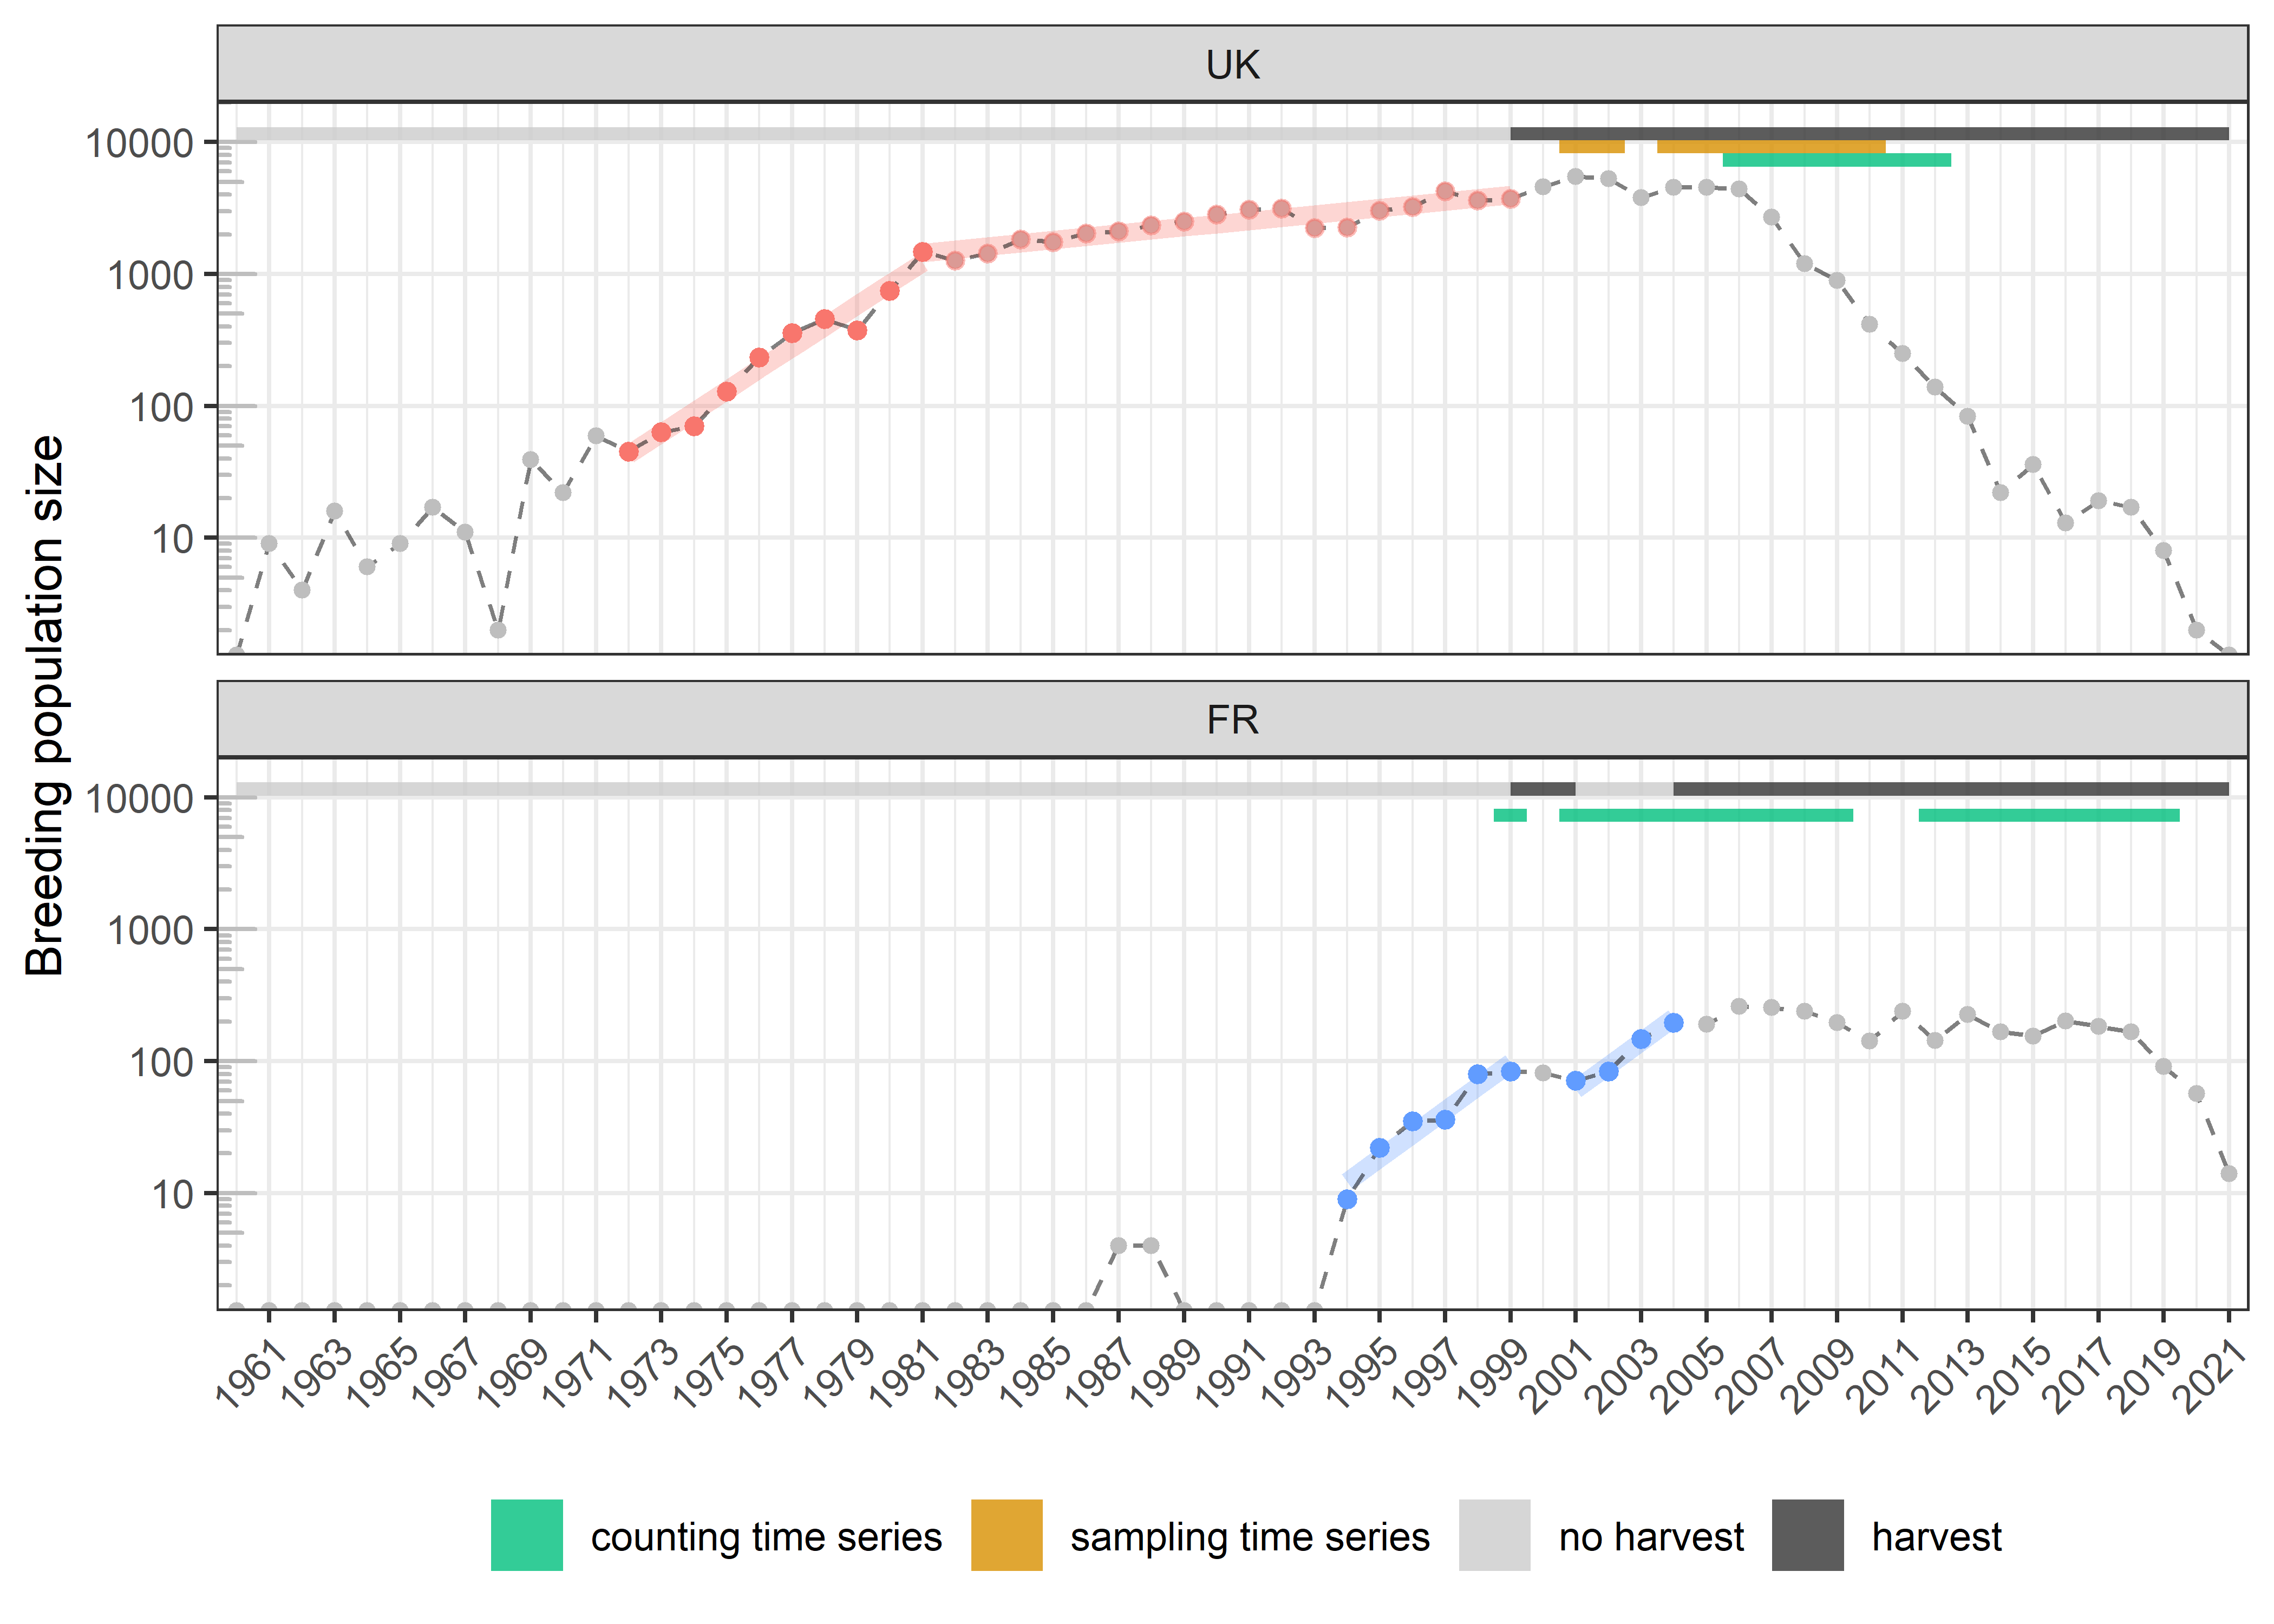
\includegraphics[width=1\linewidth]{../Output/plot_3} 

}

\caption{Evolution of the size of the two ruddy duck populations in light of the harvest pressure; on time periods without harvest, maximum population growth rates can be estimated (slopes in red for the UK and in blue for France)}\label{fig:grts}
\end{figure}

To get proxies of maximum recruitment rate from Equation \eqref{eq:GR}, one uses a very conservative prior on the adult survival by setting a uniform distribution on \([0.7; 0.9]\) (\protect\hyperlink{ref-Buxton2004}{Buxton et al., 2004}; \protect\hyperlink{ref-Krementz1997}{Krementz et al., 1997}; the lower limit corresponds to the upper range of survival rates observed in literature for species of similar weight, the upper limit corresponds to the range of survival rates of long-life species, \protect\hyperlink{ref-Nichols1997}{Nichols et al., 1997}). The average recruitment rates from the count data are estimated for each population and for each harvest category and compared to the maximum recruitment rates.

For all the sub-models in Section \ref{MM}, the Bayesian framework was used for its efficiency and simplicity to propagate error through the parameters. One generated three chains of length 500000, with a thinning of 10 to avoid autocorrelation in the samples, and one discarded the first 2000 samples as burn-in. Chain convergence was assessed using the Gelman and Rubin convergence diagnostic (R\textless1.1, \protect\hyperlink{ref-Gelman1992}{Gelman \& Rubin} (\protect\hyperlink{ref-Gelman1992}{1992})). One fit the models using NIMBLE (\protect\hyperlink{ref-Valpine2017}{de Valpine et al., 2017}) run from R (\protect\hyperlink{ref-RCT2020}{R Core Team, 2020}). Data and code are available here: \url{https://github.com/adri-tab/Ruddy_duck_recruitment_rate}. The values \emph{X{[}Y; Z{]}} reported in results are the medians and the associated boundaries of the 95\% confidence interval of posterior distributions. The median was preferred to the mean because of its robustness to skewed distribution.

\hypertarget{results}{%
\section{Results}\label{results}}

\hypertarget{recruitment-rate-variability}{%
\subsection{Recruitment rate variability}\label{recruitment-rate-variability}}

The adult male proportion, which is necessary to infer on the recruitment rate from count data, is estimated at 0.60 {[}0.59; 0.61{]}. The counting method provides estimations of the recruitment rate, see Figure \ref{fig:rrts}A. In UK, values vary from 0.06 {[}0.05; 0.07{]} to 0.27 {[}0.20; 0.34{]} recruits per breeder, and in France, 0.08 {[}0.04; 0.12{]} to 0.76 {[}0.64; 0.88{]} recruits per breeder. There are significant year-to-year variations with a maximum amplitude of 0.68 recruits per breeder in France (9.5-time variability). On the available period, recruitment rate in UK is smaller than in France. Recruitment rates are estimated in both populations over 5 years, and no correlation is observed between the two populations. The lowest recruitment rate observed in France, which is in 2019, corresponds to the start of the depletion of the population. It is noticeable that it is in the same range than the UK values, also estimated during a strong population depletion.

Recruitment rates estimated from UK sample data are consistently higher than estimates from the corresponding count data, Figure \ref{fig:rrts}A. The correlation between the two methods is strong and points out that the sampling method overestimates the recruitment rate by 44\% compared to the counting method, Figure \ref{fig:rrts}B. Estimation precision is similar for the two methods. The UK population started to deplete from 2006, but no significant shift is observed between the two periods.

\begin{figure}[H]

{\centering 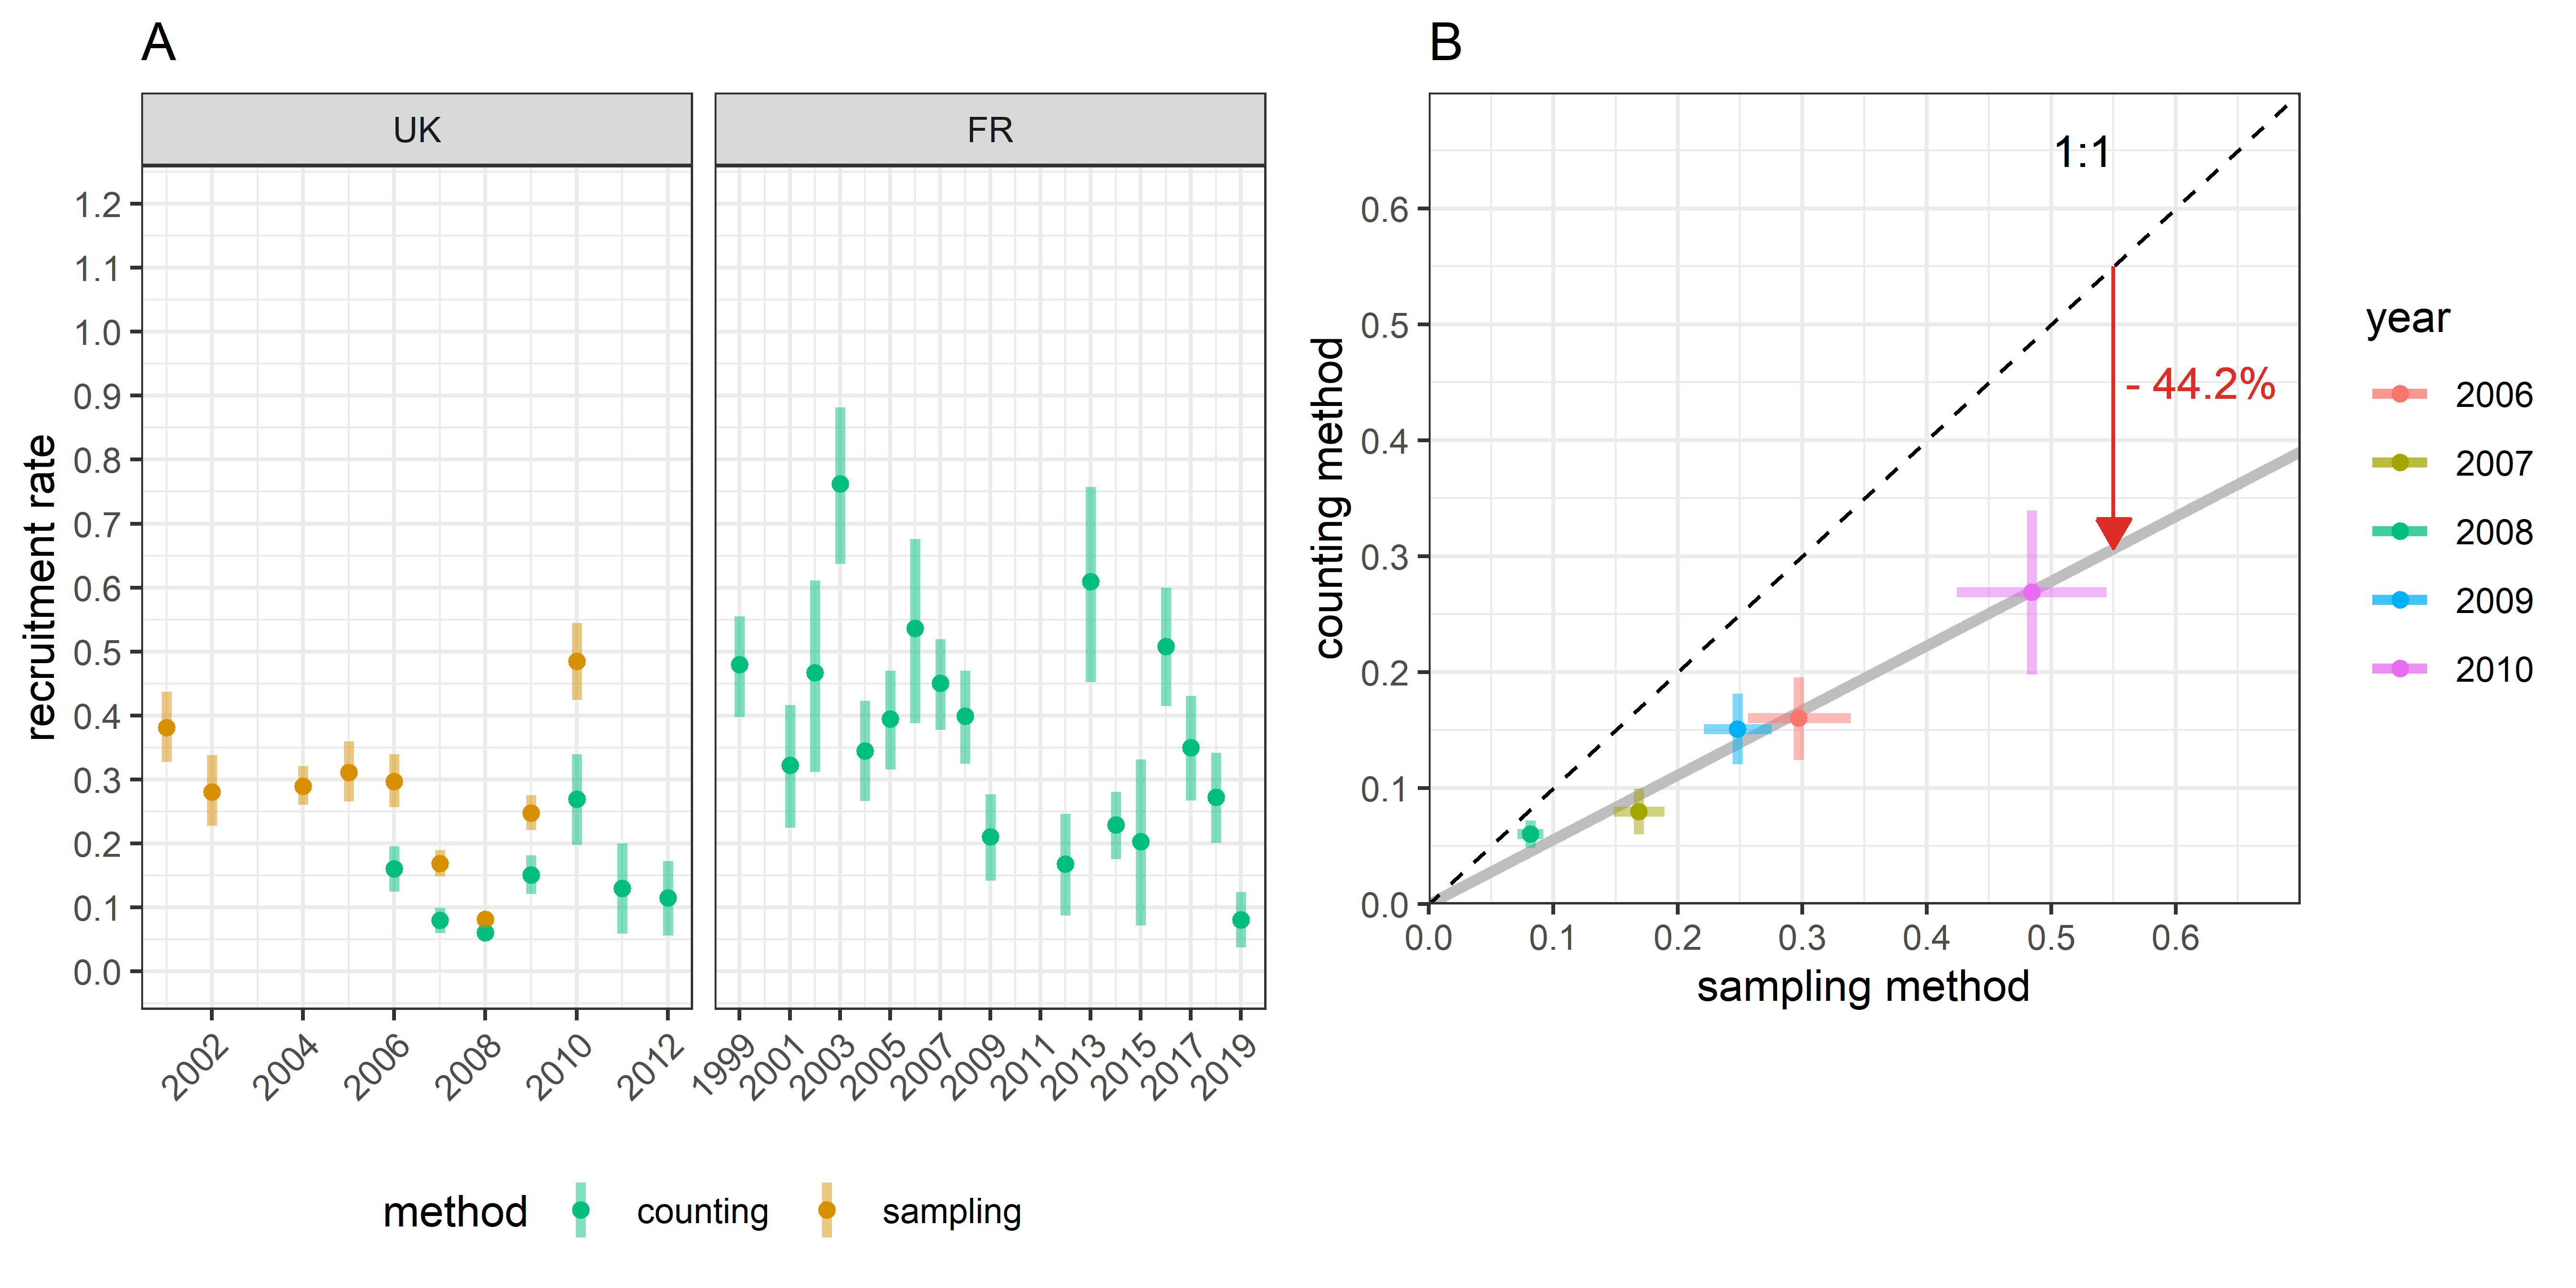
\includegraphics[width=1\linewidth]{../Output/plot_4} 

}

\caption{(A) Estimates of recruitment rate, i.e.~average number of recruits produced per breeder; (B) Comparison of the recruitment rate values between the two estimation methods; bars define the 95\% confidence intervals}\label{fig:rrts}
\end{figure}

\hypertarget{consistency-of-the-corresponding-adult-survival}{%
\subsection{Consistency of the corresponding adult survival}\label{consistency-of-the-corresponding-adult-survival}}

Adult survival rates were deduced from the recruitment rate estimates and the observed population growth rates, see Figure \ref{fig:srts}A. In UK, values that are obtained from the counting method ranged from 0.21 {[}0.20; 0.22{]} to 0.68 {[}0.65; 0.72{]}. In France, survival rates vary from 0.39 {[}0.34; 0.44{]} to 1.08 {[}0.98; 1.17{]}. Like recruitment rates, there is significant year-to-year variability without clear temporal structure in both populations with a maximum amplitude of 0.69 in France (2.8-time variability). Unlike the recruitment rate, the survival rate in 2019 in France is not a low outlier.

As expected, survival rates estimated from UK sample data are consistently lower than estimates from the corresponding count data, Figure \ref{fig:srts}A. The correlation between the two methods points out that the sampling method underestimates the survival rate by 32\% compared to the counting method, Figure \ref{fig:srts}B. Estimation precision is similar for the two methods. The sample time series shows that the adult survival is significantly lower after 2006, which corresponds to the start of the depletion of the UK population.

\begin{figure}[H]

{\centering 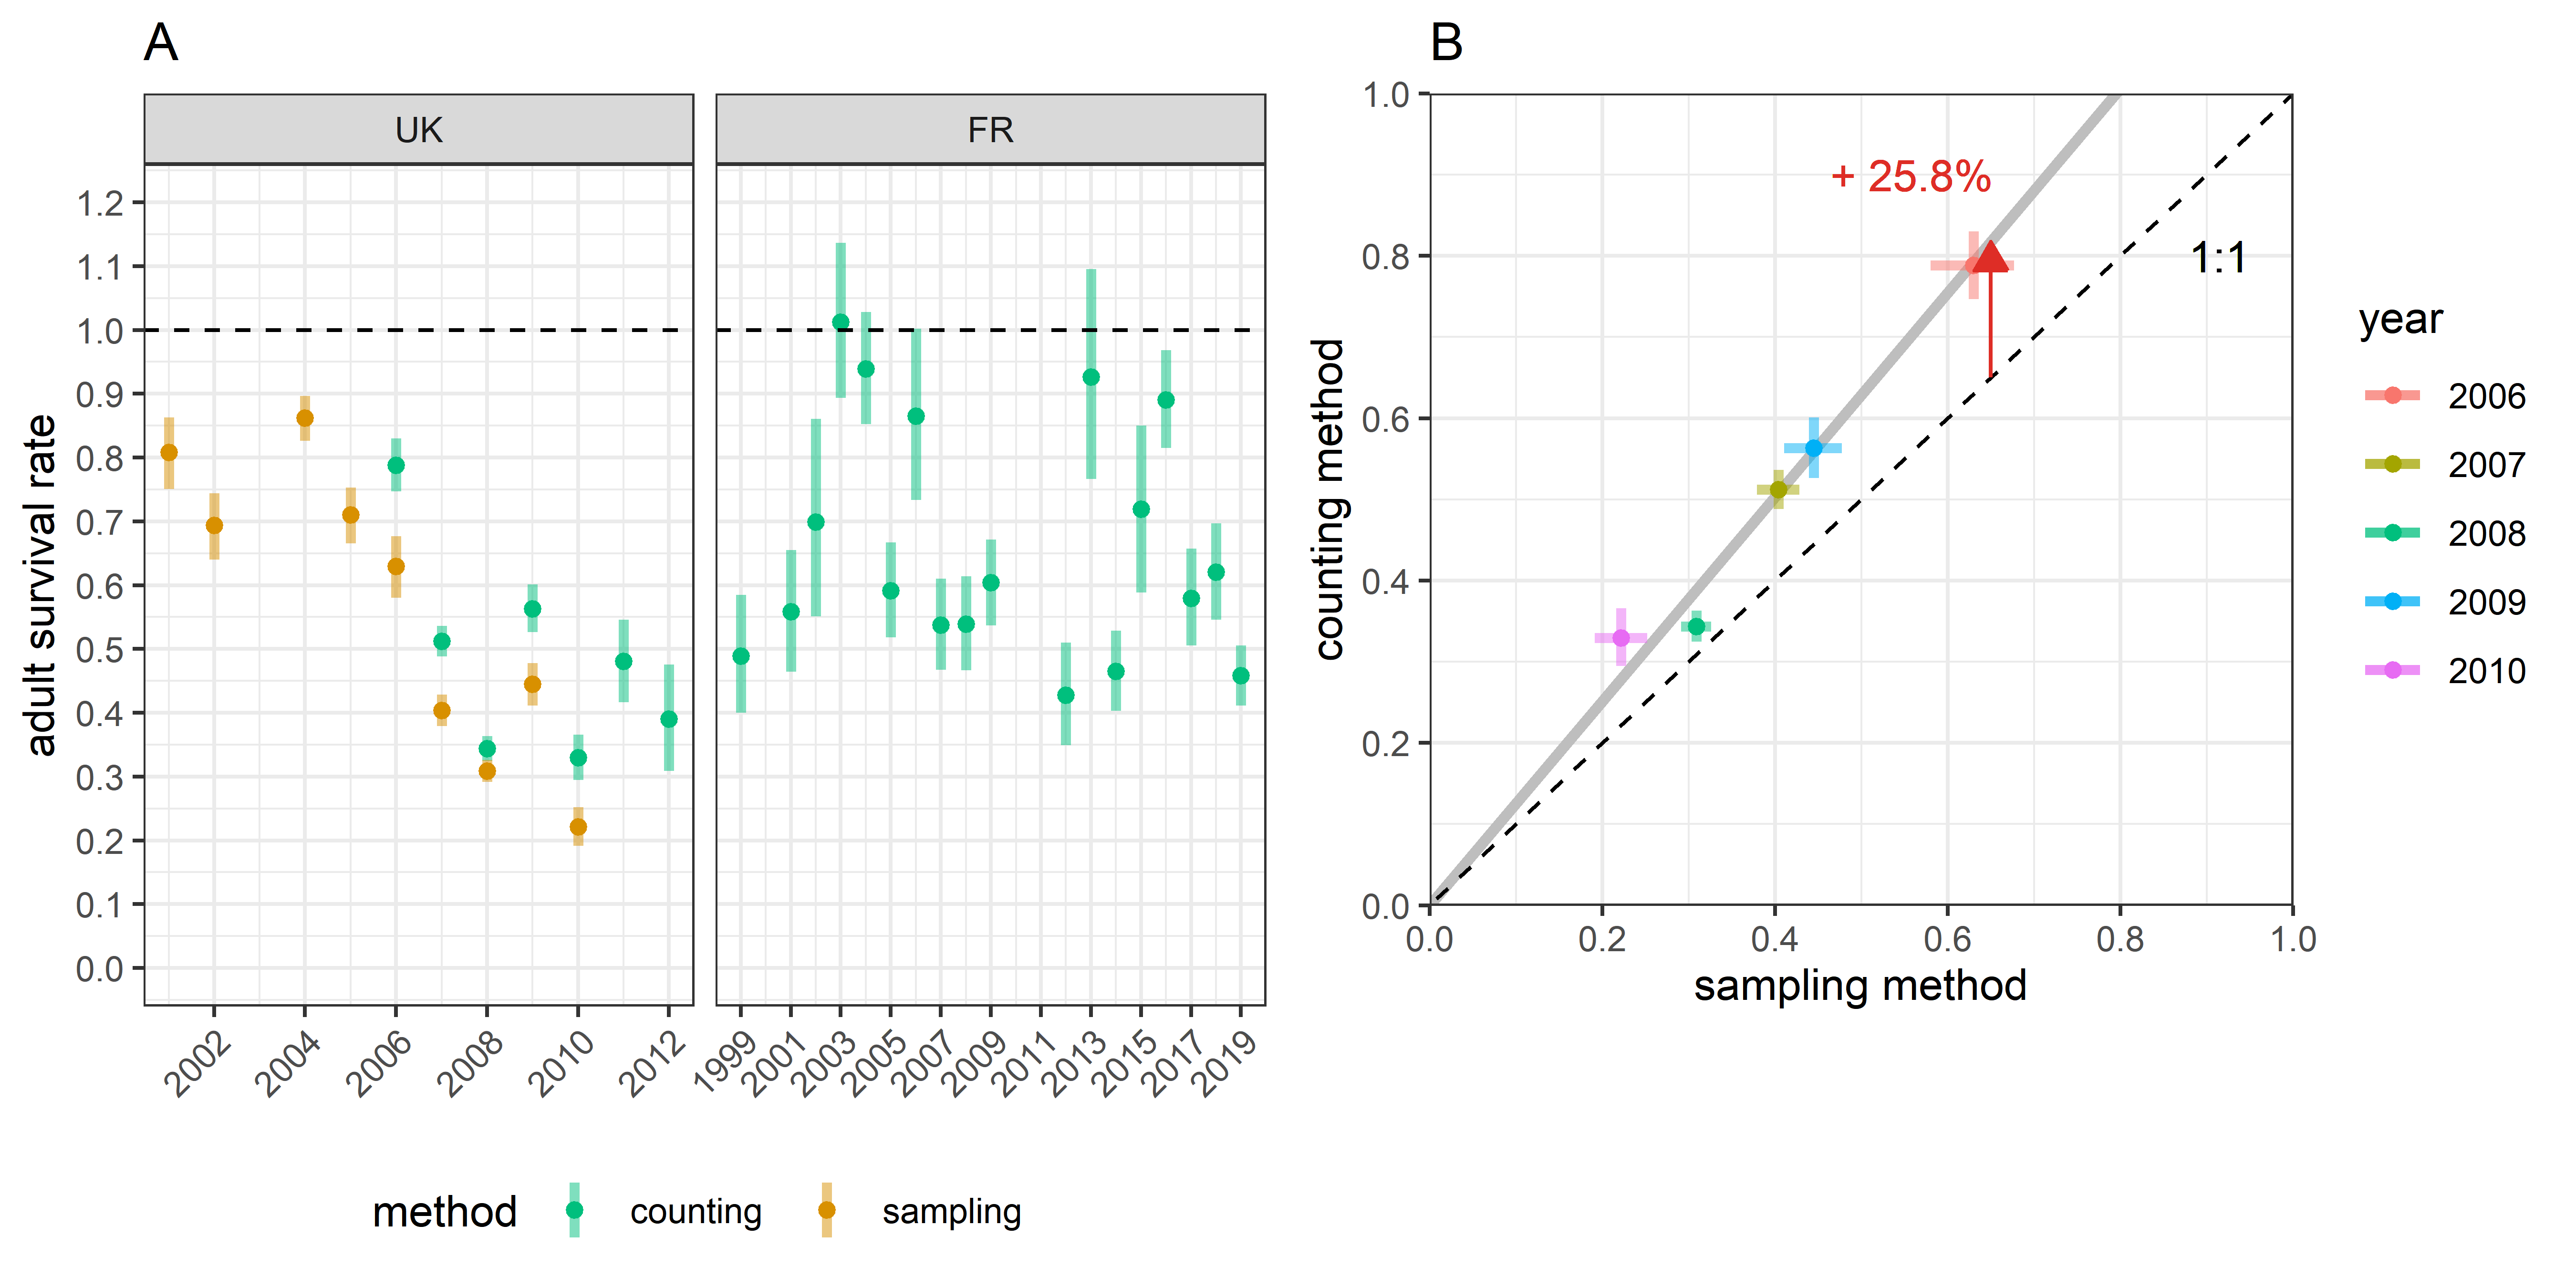
\includegraphics[width=1\linewidth]{../Output/plot_5} 

}

\caption{(A) Estimates of adult survival rate using population growth rates; (B) Comparison of the survival rate values between the two estimation methods; bars define the 95\% confidence intervals}\label{fig:srts}
\end{figure}

\hypertarget{comparison-to-a-proxy-of-maximum-recruitment-rate-1}{%
\subsection{Comparison to a proxy of maximum recruitment rate}\label{comparison-to-a-proxy-of-maximum-recruitment-rate-1}}

Maximum population growth rates are similar for the two populations, 1.45 {[}1.36; 1.55{]} and 1.47 {[}1.29; 1.68{]} for UK and France respectively, which corresponds to an increase of about 45\% per year (Figure \ref{fig:mgr}). After reaching a certain size (\textasciitilde{} 1000 individuals), the UK population growth rate falls to 1.06 {[}1.04; 1.07{]}, which corresponds to an increase of 6\% per year, even though no harvest pressure was applied on it.

\begin{figure}[H]

{\centering 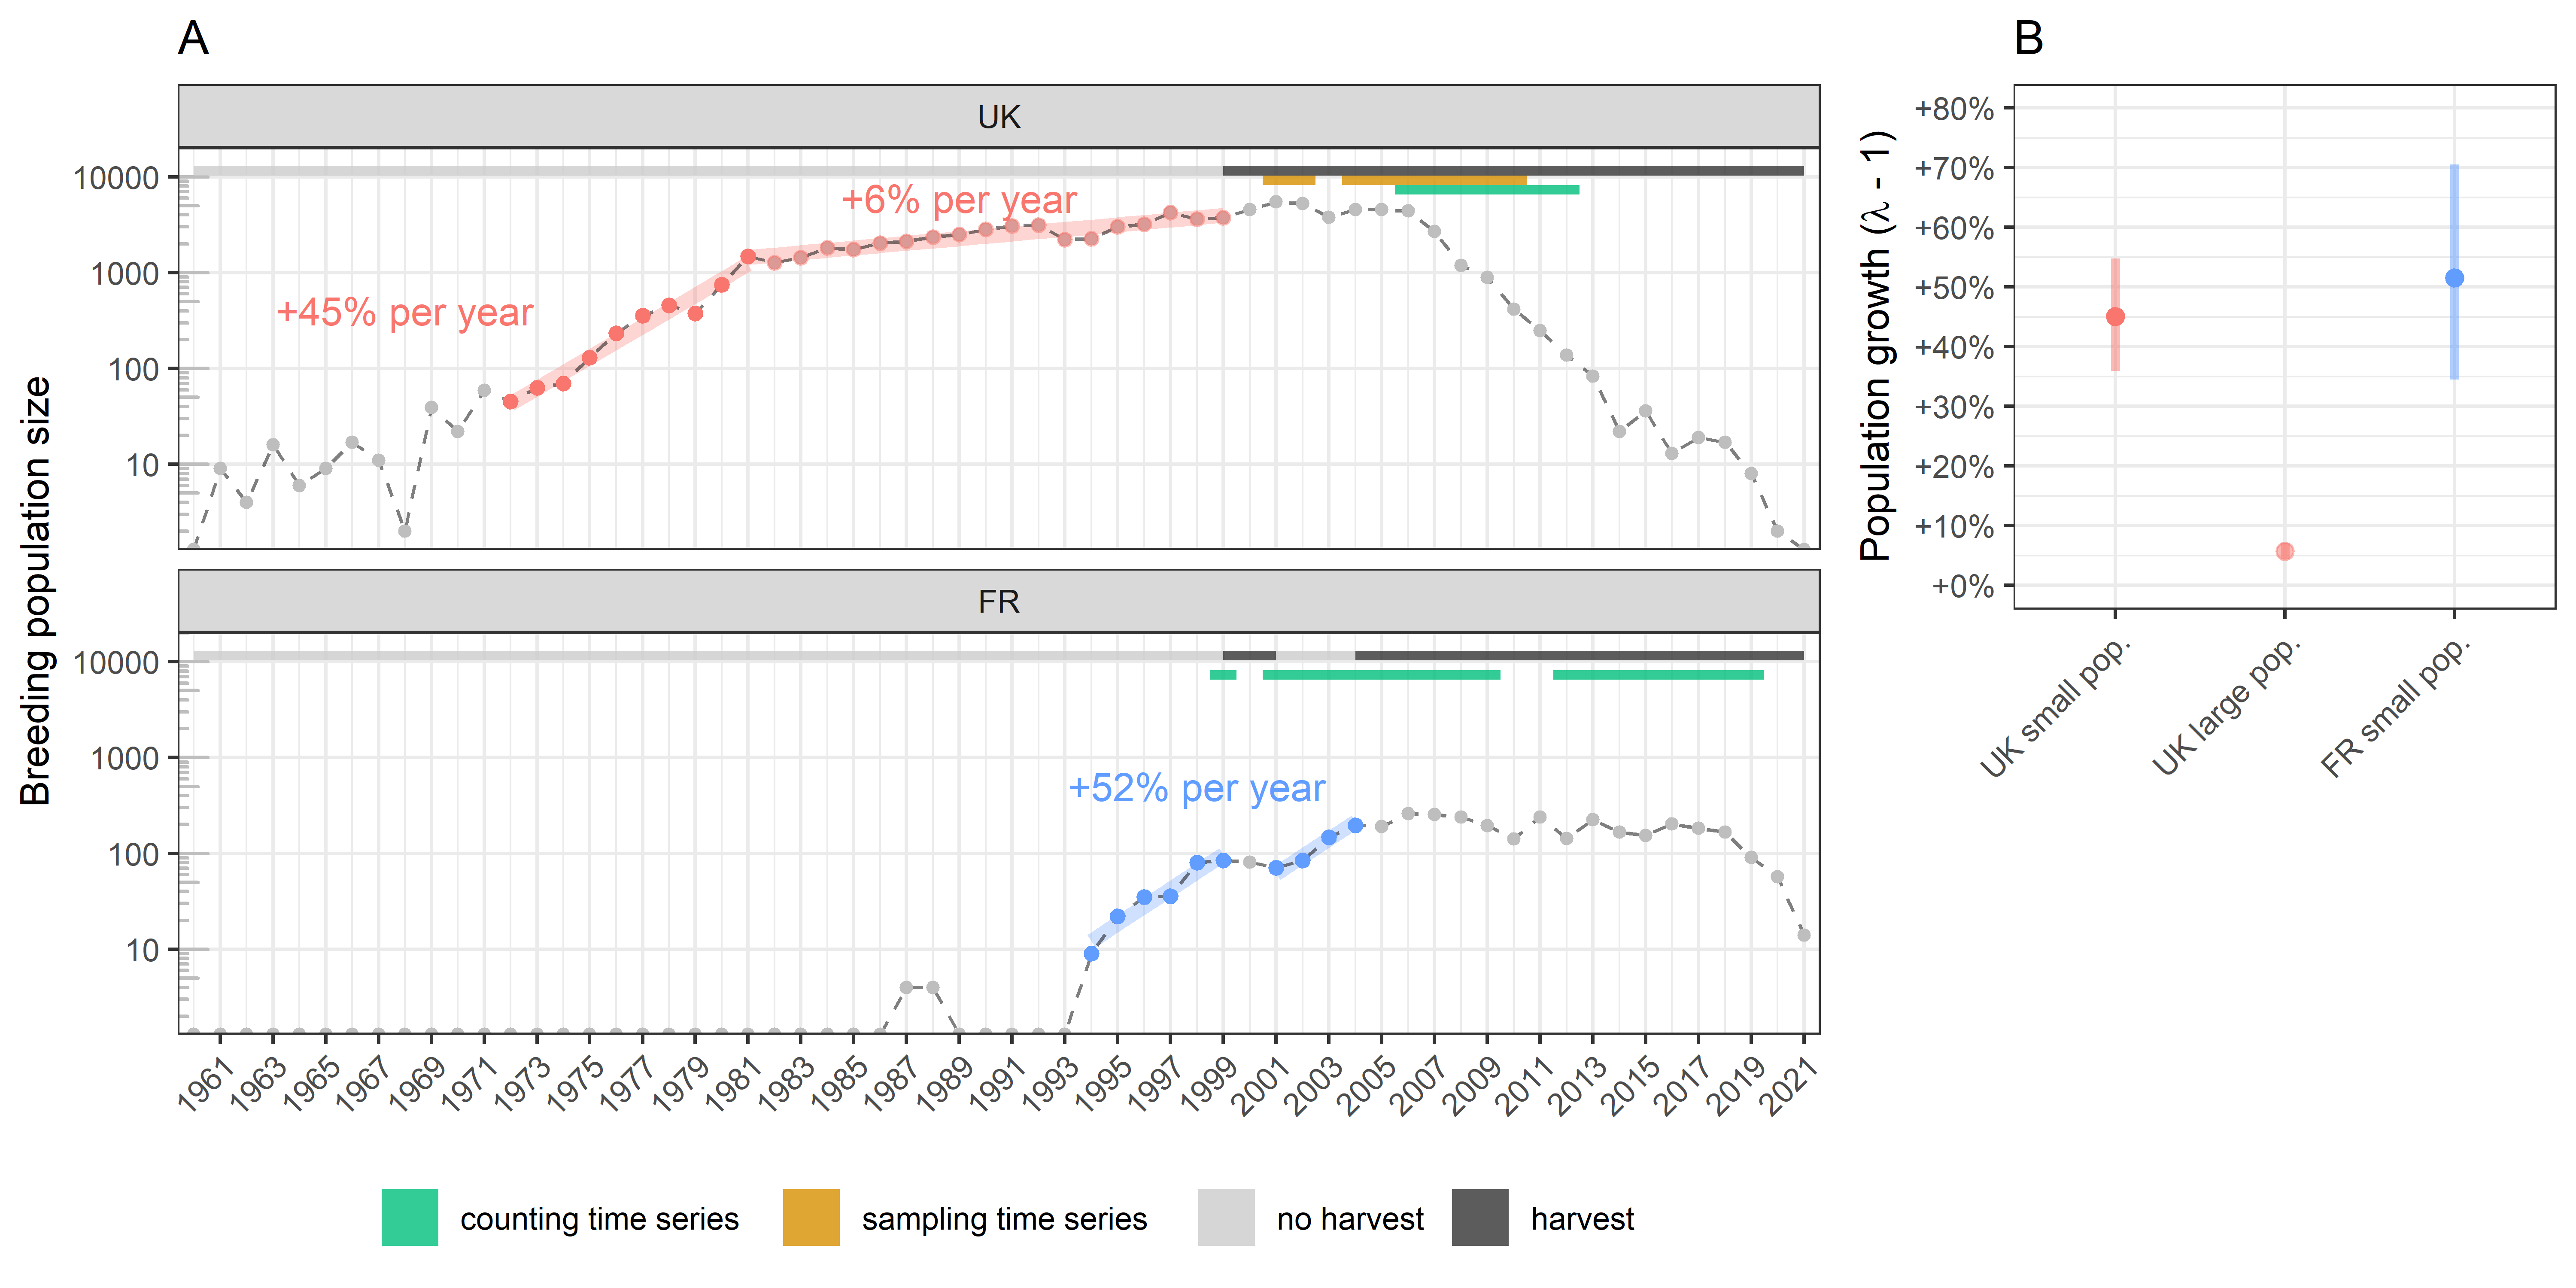
\includegraphics[width=1\linewidth]{../Output/plot_6} 

}

\caption{(A) Estimates of the maximum population growth without harvest \((\lambda - 1)\); two estimates were produced for the UK population because the growth rate dropped significantly when its size reached more than 1000 individuals; (B) Growth rate estimates; bars define the 95\% confidence intervals}\label{fig:mgr}
\end{figure}

Upon the conservative assumption of a maximum adult survival uniformly distributed over 0.70 to 0.90, the maximum recruitment rate reaches 0.65 {[}0.51; 0.75{]} and 0.66 {[}0.45; 0.90{]} recruits per breeder for UK and France respectively (Figure \ref{fig:grcomp}). When there is no harvest, the estimated average recruitment rate of the French population is in the range of the proxy of the maximum recruitment rate, 0.51 {[}0.46; 0.57{]} recruits per breeder. When there is harvest, the average recruitment rates are 0.14 {[}0.12; 0.16{]} and 0.33 {[}0.31; 0.36{]} recruits per breeder for the UK and France respectively. Both values are significantly lower than the maximum recruitment rate, and it is noticeable that the average recruitment rate is lower for the UK population, which is in depletion over the count time series, than for the French population, which of the dynamic is mostly stable over the monitored period.

\begin{figure}[H]

{\centering 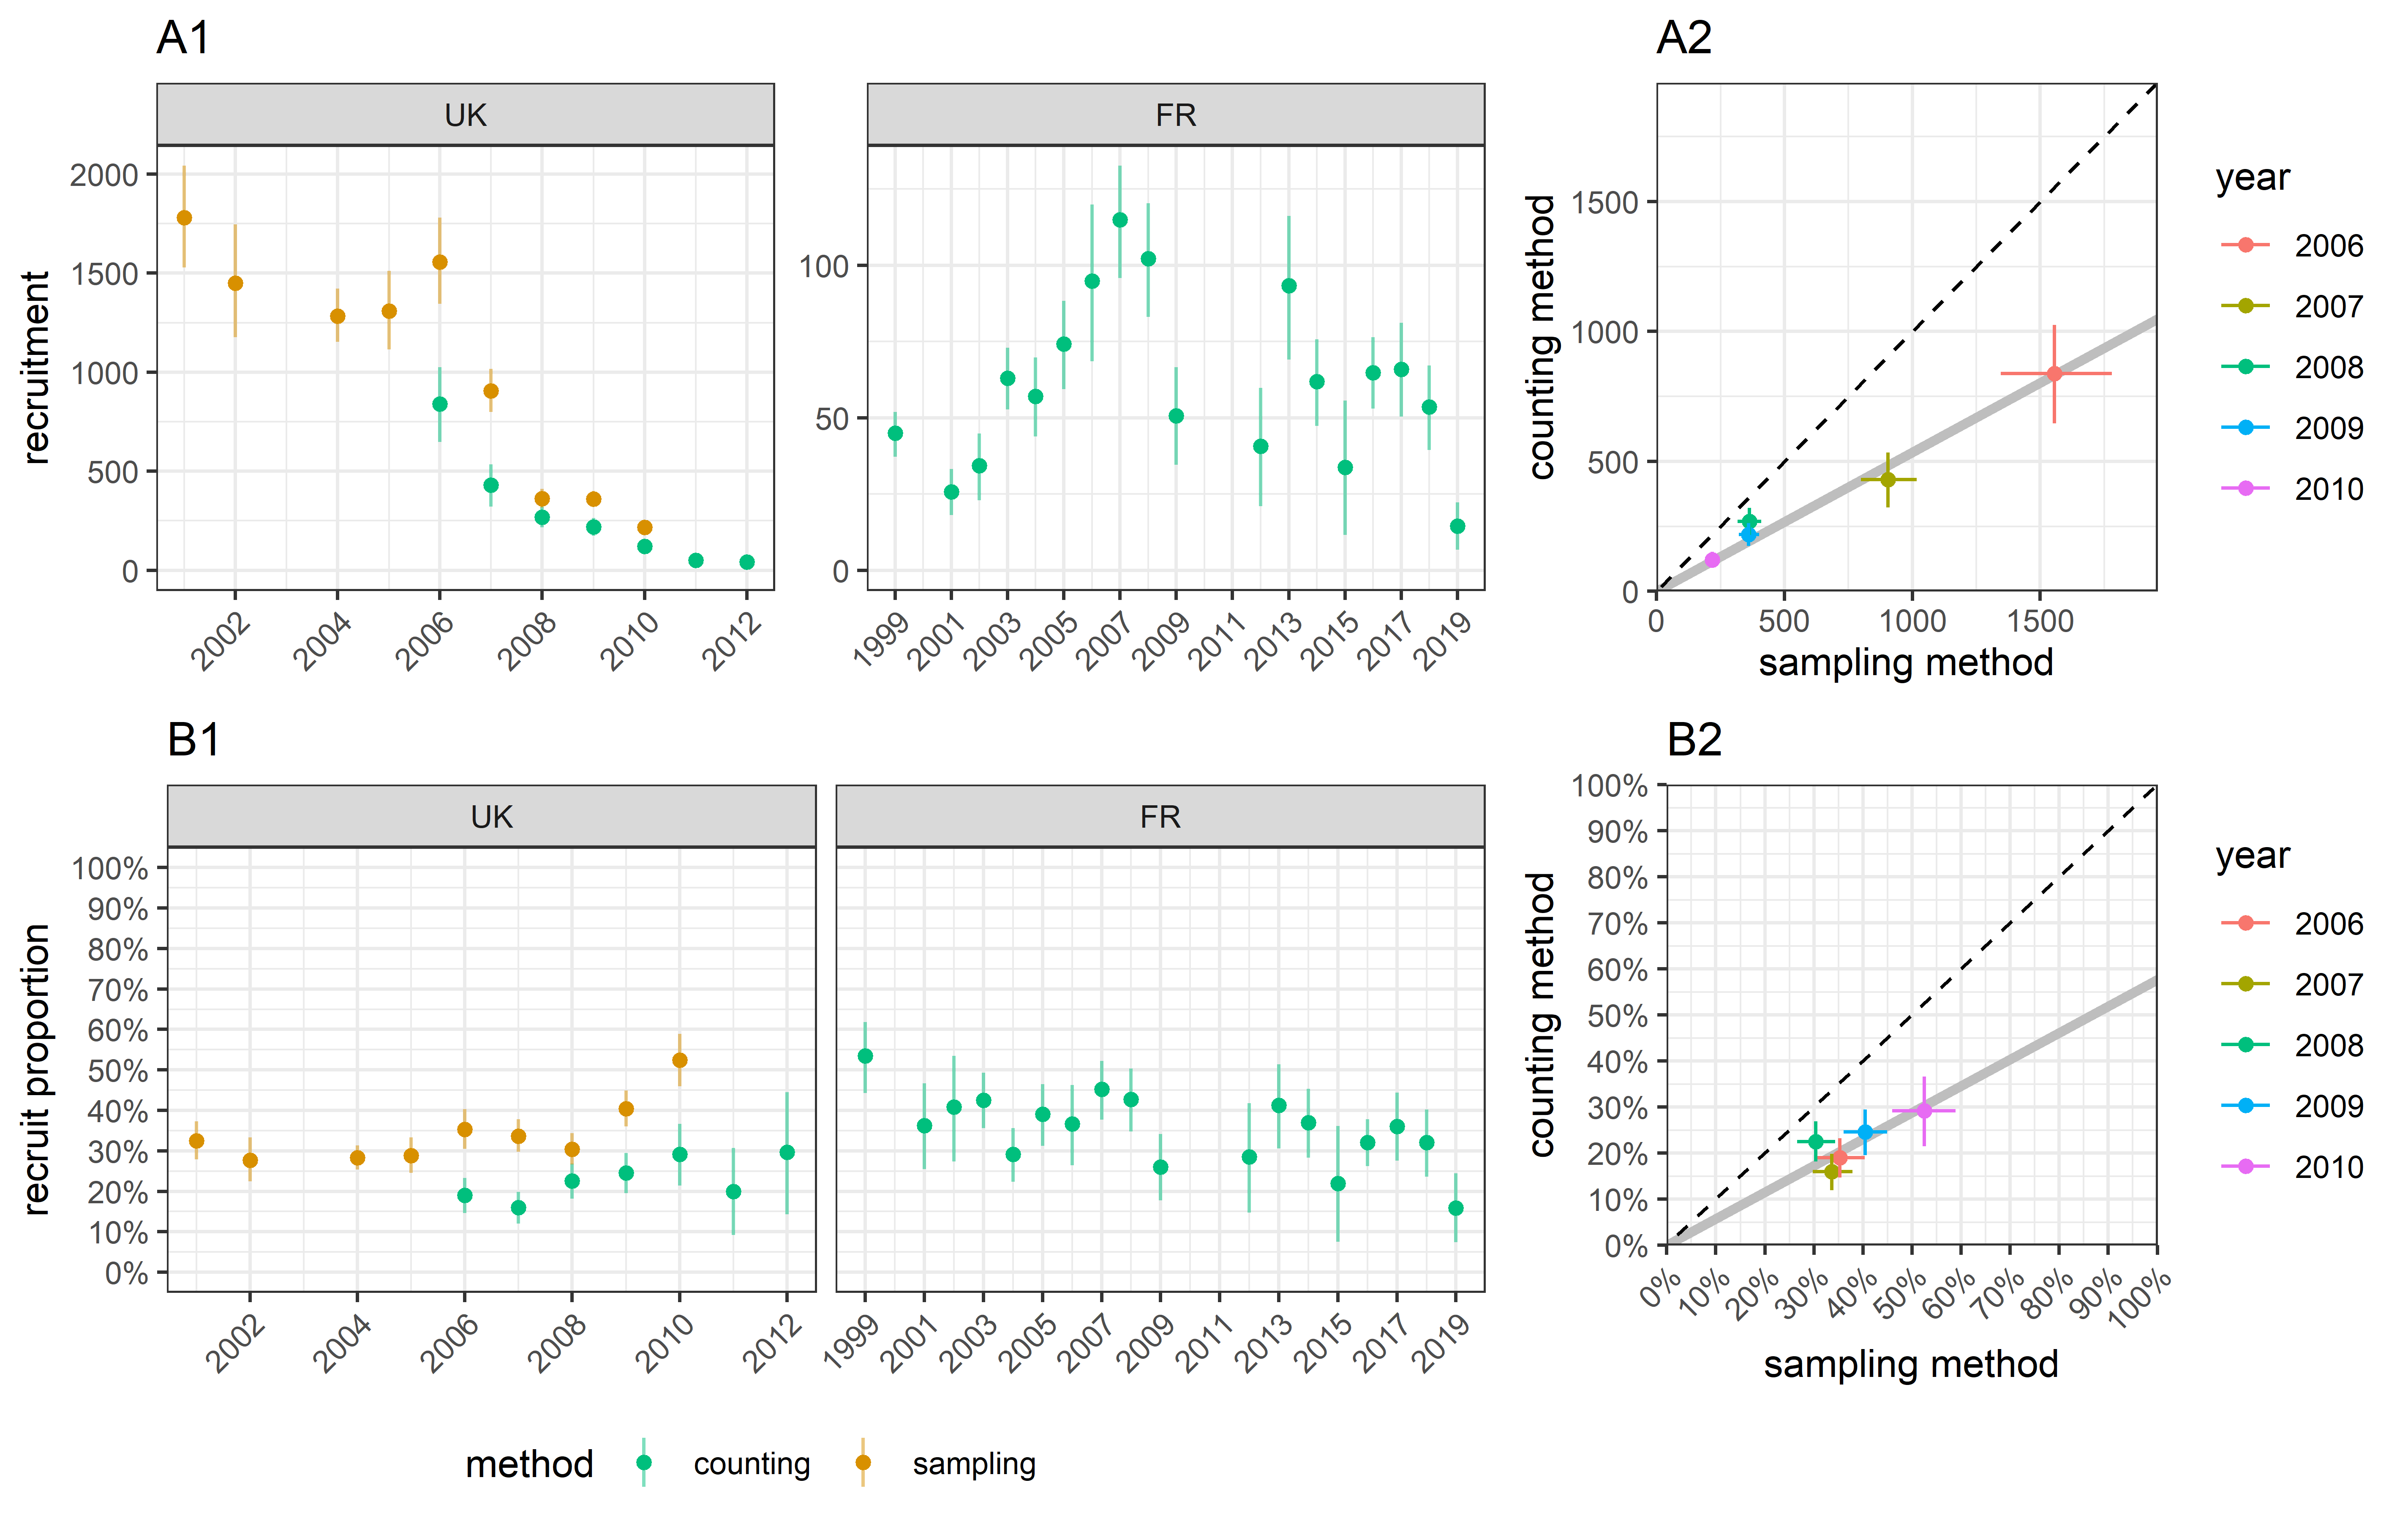
\includegraphics[width=1\linewidth]{../Output/plot_7} 

}

\caption{Comparison between proxies of maximum recruitment rate and average recruitment rates estimated with and without harvest (\emph{counting} method only); proxies are estimated by using the maximum growth rates; bars define the 95\% confidence intervals}\label{fig:grcomp}
\end{figure}

\hypertarget{discussion}{%
\section{Discussion}\label{discussion}}

Count data in waterfowl that differentiate adult males from other individuals are successfully used in this study to infer estimations of recruitment rates. In the following section, one checks the accuracy of the method from indicators developed for this purpose. From the outputs on the two populations of ruddy duck, one discusses about the effects of the harvest on the recruitment rate and its implication on waterfowl management.

\hypertarget{accuracy-of-the-counting-method}{%
\subsection{Accuracy of the counting method}\label{accuracy-of-the-counting-method}}

The recruitment rates from the counting method vary in the same range for the two populations, which demonstrate a certain robustness of the method. The higher variability observed in France is not unexpected because the French time series is longer and covers a larger harvest spectrum than in UK. There is no temporal correlation between the two populations, so it suggests that the recruitment rate fluctuations are more likely influenced by regional-scale factors than large-scale ones. This is consistent with the literature because both nesting/hatching success and juvenile survival are conditional to the onset of lay, which is tightly related to local weather parameters, e.g.~the spring temperature, the cumulative rainfall, and the water levels (\protect\hyperlink{ref-Blums2004}{Blums \& Clark, 2004}; \protect\hyperlink{ref-Dzus1998}{Dzus \& Clark, 1998}; \protect\hyperlink{ref-Folliot2017}{Folliot et al., 2017}).

Assuming that the sample data provide a good picture of the interannual variability of the recruitment rate, the good correlation to the outputs of the counting method demonstrates the ability of this method to track the recruitment rate variability. This result is quite robust because the correlation is obvious with only a five-year time series. However, this conclusion might be overrated because two successive population size values are part of the recruitment rate, which mechanically scale the outputs. It explains why the correlation on the immature proportion, the other component of the recruitment rate, is a bit more noisy than for the recruitment rate (Figure \ref{fig:sup}A). The uncertainty of the estimates is very close to the outputs from the sampling method. Even though the counting method is more indirect to infer on the recruitment rate, it performs to provide a good confidence of the outputs which is satisfying.

A significant change in adult sex ratio would bias the estimation of recruitment rate. However, since this ratio integrates many age-cohorts, the temporal autocorrelation is structurally strong. Significant variations can then occur only every multiple years, especially if it is a long-living species. Consequently, it is not necessary to monitor and update the adult sex ratio on a yearly base.

The counting method always provides recruitment rates significantly lower than the sampling method by factor close to 2 on average, a result that is in line with the hypothesis that the harvest is generally selective towards immature individuals in waterfowl because they are more vulnerable to hunters (\protect\hyperlink{ref-Bellrose1980}{Bellrose, 1980}; \protect\hyperlink{ref-Fox2014}{A. D. Fox et al., 2014}). This is a robust result because the approaches used to control ruddy ducks differ strongly from usual hunting practices and are apriori less selective. It is especially clear in the UK, for which control operations occur in winter using long-range rifles that prevents the bird from escaping from the threat. The assumption on the accuracy of the counting method is then not excluded from the consistency of this result.

Annual adult survival rates deduced from observed population growth rates and recruitment estimates are on average in line with the literature \textbf{ref required}. which confirms that the counting method is poorly biased if there is some bias.

survival in the range of the expected values -\textgreater{} so no apparent issue of scaling issue,
so we the hypothesis that male-like individuals corresponds only to adult male is validated.

\emph{average recruitment rate compared to a proxy of maximum recruitment rate}

always below the maximum recruitment rate so satisfying.

overall, even if we don't have access to the true value of the recruitment rate to test the accuracy of the counting method, a beam of arguments support that the method is not heavily biased, unlike the sampling method, as demonstrated in \protect\hyperlink{ref-Fox2014}{A. D. Fox et al.} (\protect\hyperlink{ref-Fox2014}{2014}), even if one considers a picture limited to the end of the hunting season (\protect\hyperlink{ref-Fox2016}{A. Fox et al., 2016}).

\hypertarget{influence-of-harvest-on-the-recruitment-rate}{%
\subsection{Influence of harvest on the recruitment rate}\label{influence-of-harvest-on-the-recruitment-rate}}

Variability within harvest category represents

\hypertarget{implication-in-waterfowl-management}{%
\subsection{Implication in waterfowl management}\label{implication-in-waterfowl-management}}

Survival higher than one but warning, observation error, so annual population growth rate might be inaccurate on some years. Also, we assumed a closed population, but it is possible that years with adult survival higher than one corresponds to an arrival of birds from the other population. As a consequence, the recruitment rate on these years may also be overestimated.

No impact on the adult survival in France, but it seems that there is an impact in UK.
Why, because harvest occurs mostly in summer in France, and in winter in UK.

The harvest pressure, simplified into a two-category variable, explains already 19.3\% and 4.6\% of the variance of the recruitment rate and the adult survival rate of the French population. The harvest pressure described as a continuous variable is expected to explain even more the recruitment rate variability. The harvest pressure applied in France is thus a factor that likely induces a strong immature mortality, but a moderate one on the adults.

Impact on the recruitment rate in France, and no impact in UK.

Overall, the harvest seems to impact differently France and UK, likely because the harvest mortality occurs mostly in summer in France, and in winter in UK.

But caution, a population model linking the harvest rate to state variables describing the population is necessary to check precisely the impact of the harvest pressure, and test hypothesis on the functioning of harvest mortality.

Recruitment rate decrease with the harvest for the French population, and the UK population recruitment rate is also below the French one.
it seems quite clear that the harvest affects the recruitment rate.

\emph{reference to introduction}

It is quite consistent with the assumption in introduction. Since studied populations are in colonization of their habitat, maximum densities are not reached, and then no or limited density dependent effect occur.

If counting method acceptable, moderate harvest pressure does not reduce the recruitment rate as expected, maybe due to density dependent mortality for juvenile but it affects it if strong harvest rate. That is very interesting bro but warning, these interpretation holds on weak estimations and adult survival equal to 1!!!

it may be possible that first sight of density dependence occur in UK from 1000 individuals, but was not big enough to fully curb the population growth. Since there is a strong correlation between the number of birds observed and the number of sites occupied by the birds, this inflexion may be simply due to a limited number of new favourable sites to be colonized.

What about heterogeneity, figure 8 -\textgreater{} One said that recruitment rate can increase if harvest because of heterogeneity and density dependence, but it is not what we observe in France, likely because the exploitation is high inhere and consequently impact.

\hypertarget{use-of-recruitment-rate}{%
\subsection{Use of recruitment rate}\label{use-of-recruitment-rate}}

\emph{better than sex ratio}
a same value of age ratio can correspond to different fecundity levels, so warning.
a same value of age ratio for a population in depletion and a population stabilized are not similary productive, the first one is less productive than the second one !
so warning, focus on recruitment rate and not on age ratio if the dynamics of the population varies! recruitment proportion is commonly used in to discuss the fecundity of a population, but unlike the recruitment rate, this indicator does not consider the dynamics of the population and does reflect fecundity only on stable growth period

the consistency between the two max growth rate strenghtens that seems to be a biological limit for this species, at least in the western Palearctic.

As described before, recruitment rate over the studied time period is far lower for the UK than France (2.5 factor).
Underlined adult survival are comprised between 0 and 1, whatever the method. So we cannot conclude if one can be rejected.

France affected the recruitment, UK affected adult survival for a similar result -\textgreater{} depletion

whereas adult survival more consistent between the tow (.5 factor), meaning there was more variability in recruitment rate than in survival rate. growth rate difference is thus more explained by recruitment rate fluctuation than adult survival fluctuation, consistent with the demographic buffering, or canalization hypothesis (\protect\hyperlink{ref-Gaillard2003}{Gaillard \& Yoccoz, 2003}; \protect\hyperlink{ref-Lenzi2021}{Lenzi et al., 2021})

survival values compared to literature? s

Abundance index are considered exact, which should not be true. and lead to structural error in the estimates of annual growth rate.

\protect\hyperlink{ref-Arnold2018}{Arnold} (\protect\hyperlink{ref-Arnold2018}{2018}) underlines the lack of data on recruitment rate for modellers (in discussion) and that new methods are required to track this variable that often drive the population growth rate

Recruitment rate drives lambda? see \protect\hyperlink{ref-Arnold2018}{Arnold} (\protect\hyperlink{ref-Arnold2018}{2018})

(only X years), meaning no large scale factor drive the fluctuations of productivity.

adult sex ratio in line with other duck species (\protect\hyperlink{ref-Wood2021}{Wood et al., 2021})

This time lag might be not a issue if the survival of immature is close to the adult survival between the two periods. winter count and breeding season

According to \protect\hyperlink{ref-Blums2004}{Blums \& Clark} (\protect\hyperlink{ref-Blums2004}{2004}), the recruitment for diving ducks is not related to the fecundity, but depends mostly on the juvenile survival, which is driven by weather conditions. Studies on other birds also conclude of the poor correlation between fecundity and recruitment (e.g. \protect\hyperlink{ref-Murray2000}{Murray, 2000}).

No correlation between the two populations on recruitment rate, so maybe no large scale drivers of recruitment rate variability.

age proportion -\textgreater{} {[}0, 1{]}
recruitment rate {[}0, +inf{]} donc plus sensitive

recruitment rate the most sensitive parameter to density dependent effect (\protect\hyperlink{ref-Koons2014}{Koons et al., 2014})

Hypothesis of time invariant sex ratios in immature and adult: limits

For hunted duck species in North America, the mortality rate on first-year immatures compared to adults is higher by a factor ranging from 1.4 to 2 (Bellrose 1980).

recruitment rate:
Stabilité grosse pop,
variabilité petite pop.

Au dela du fait que la croissance de la pop est la somme de la survie et de la recruitment rate,
intéressant de parler de la variability de la survie vs variabilité de la recruitment rate
pour parler de risk management.

recruitment rate: drop from 2009

one considers harvest as an impact only adult survival, not on age structure, but we should, oversimplistics

blabla

\protect\hyperlink{ref-Nichols2006}{Nichols \& Williams} (\protect\hyperlink{ref-Nichols2006}{2006}) -\textgreater{} il faut compter de la façon dont on demande

Taper des jeunes c'est pas forcément très utile car density dependence

If the maximum recruitment rate is not reached under optimal conditions (maximum population size not reached, and limited harvest pressure), it is a signal that one should explore the intermediate life stages before recruitment to provide a diagnostic on the changes of the environment conditions that have affected the recruitment rate.

Condition of application to other species.

Message de l'article

\hypertarget{acknowledgments}{%
\section*{Acknowledgments}\label{acknowledgments}}
\addcontentsline{toc}{section}{Acknowledgments}

This work was partly funded by the LIFE Oxyura project (LIFE17 NAT/FR/000942) through the LIFE program. This work was carried on with the impulse of Jean-François Maillard, and Jean-Baptiste Mouronval from the \emph{Office Français de la Biodiversité}, and Jean-Marc Gillier from the \emph{Société Nationale pour la Protection de la Nature}. The authors acknowledge all the contributors of the data collection in the UK and in France, especially: \textbf{UK names}, Vincent Fontaine, Denis Lacourpaille, Justin Potier, Alexis Laroche, Médéric Lortion, Jules Joly, and Valentin Boniface.

\hypertarget{references}{%
\section*{References}\label{references}}
\addcontentsline{toc}{section}{References}

\hypertarget{refs}{}
\begin{CSLReferences}{1}{0}
\leavevmode\vadjust pre{\hypertarget{ref-Anders2005}{}}%
Anders, A. D., \& Marshall, M. R. (2005). Increasing the accuracy of productivity and survival estimates in assessing landbird population status. \emph{Conservation Biology}, \emph{19}(1), 66--74.

\leavevmode\vadjust pre{\hypertarget{ref-Arnold2018}{}}%
Arnold, T. W. (2018). Using ring-recovery and within-season recapture data to estimate fecundity and population growth. \emph{Ecology and Evolution}, \emph{8}(20), 10298--10305. \url{https://doi.org/10.1002/ece3.4506}

\leavevmode\vadjust pre{\hypertarget{ref-Bellrose1980}{}}%
Bellrose, F. C. (1980). \emph{Ducks, geese \& swans of {N}orth {A}merica: 3rd. ed}. Stackpole Books.

\leavevmode\vadjust pre{\hypertarget{ref-Blums2004}{}}%
Blums, P., \& Clark, R. G. (2004). Correlates of lifetime reproductive success in three species of {E}uropean ducks. \emph{Oecologia}, \emph{140}(1), 61--67. \url{https://doi.org/10.1007/s00442-004-1573-8}

\leavevmode\vadjust pre{\hypertarget{ref-Buxton2004}{}}%
Buxton, N. E., Summers, R. W., \& Peach, W. J. (2004). Survival rate of female \emph{{B}oldeneye bucephala} clangula. \emph{Bird Study}, \emph{51}(3), 280--281. \url{https://doi.org/10.1080/00063650409461365}

\leavevmode\vadjust pre{\hypertarget{ref-Cooch2014}{}}%
Cooch, E. G., Guillemain, M., Boomer, G. S., Lebreton, J.-D., \& Nichols, J. D. (2014). The effects of harvest on waterfowl populations. \emph{Wildfowl}, 220--276.

\leavevmode\vadjust pre{\hypertarget{ref-Valpine2017}{}}%
de Valpine, P., Turek, D., Paciorek, C. J., Anderson-Bergman, C., Lang, D. T., \& Bodik, R. (2017). Programming with models: Writing statistical algorithms for general model structures with {NIMBLE}. \emph{Journal of Computational and Graphical Statistics}, \emph{26}(2), 403--413. \url{https://doi.org/10.1080/10618600.2016.1172487}

\leavevmode\vadjust pre{\hypertarget{ref-Dzus1998}{}}%
Dzus, E. H., \& Clark, R. G. (1998). Brood survival and recruitment of mallards in relation to wetland density and hatching date. \emph{The Auk}, \emph{115}(2), 311--318. \url{https://doi.org/10.2307/4089189}

\leavevmode\vadjust pre{\hypertarget{ref-Eraud2021}{}}%
Eraud, C., Devaux, T., Villers, A., Johnson, F. A., \& Francesiaz, C. (2021). Popharvest: An {R} package to assess the sustainability of harvesting regimes of bird populations. \emph{Ecology and Evolution}. \url{https://doi.org/10.1002/ece3.8212}

\leavevmode\vadjust pre{\hypertarget{ref-Etterson2011}{}}%
Etterson, M. A., Ellis-Felege, S. N., Evers, D., Gauthier, G., Grzybowski, J. A., Mattsson, B. J., Nagy, L. R., Olsen, B. J., Pease, C. M., Burg, M. P. van der, \& Potvien, A. (2011). Modeling fecundity in birds: Conceptual overview, current models, and considerations for future developments. \emph{Ecological Modelling}, \emph{222}(14), 2178--2190. \url{https://doi.org/10.1016/j.ecolmodel.2010.10.013}

\leavevmode\vadjust pre{\hypertarget{ref-Flint2015}{}}%
Flint, P. (2015). Population dynamics of sea ducks: Using models to understand the causes, consequences, evolution, and management of variation in life history characteristics. In J.-P. L. Savard, D. V. Derksen, D. Esler, \& J. M. Eadie (Eds.), \emph{Ecology and conservation of {N}orth {A}merican sea ducks} (Vol. 46, pp. 63--96). CRC Press.

\leavevmode\vadjust pre{\hypertarget{ref-Folliot2017}{}}%
Folliot, B., Caizergues, A., Barbotin, A., \& Guillemain, M. (2017). Environmental and individual correlates of common pochard (\emph{{A}ythya ferina}) nesting success. \emph{European Journal of Wildlife Research}, \emph{63}(4). \url{https://doi.org/10.1007/s10344-017-1126-1}

\leavevmode\vadjust pre{\hypertarget{ref-Fox2014}{}}%
Fox, A. D., Clausen, K. K., Dalby, L., Christensen, T. K., \& Sunde, P. (2014). Age-ratio bias among hunter-based surveys of {E}urasian wigeon \emph{{A}nas penelope} based on wing vs. Field samples. \emph{Ibis}, \emph{157}(2), 391--395. \url{https://doi.org/10.1111/ibi.12229}

\leavevmode\vadjust pre{\hypertarget{ref-Fox2016}{}}%
Fox, A., Clausen, K., Dalby, L., Christensen, T., \& Sunde, P. (2016). Between-year variations in sex/age ratio bias in hunter wings of eurasian wigeon (\emph{{A}nas penelope}) compared to field samples. \emph{Ornis Fennica}, \emph{93}(1), 26.

\leavevmode\vadjust pre{\hypertarget{ref-Gaillard2003}{}}%
Gaillard, J.-M., \& Yoccoz, N. G. (2003). {TEMPORAL} {VARIATION} {IN} {SURVIVAL} {OF} {MAMMALS}: A {CASE} {OF} {ENVIRONMENTAL} {CANALIZATION}? \emph{Ecology}, \emph{84}(12), 3294--3306. \url{https://doi.org/10.1890/02-0409}

\leavevmode\vadjust pre{\hypertarget{ref-Gelman1992}{}}%
Gelman, A., \& Rubin, D. B. (1992). Inference from iterative simulation using multiple sequences. \emph{Statistical Science}, \emph{7}(4). \url{https://doi.org/10.1214/ss/1177011136}

\leavevmode\vadjust pre{\hypertarget{ref-Gimenez2017}{}}%
Gimenez, O., Cam, E., \& Gaillard, J.-M. (2017). Individual heterogeneity and capture-recapture models: What, why and how? \emph{Oikos}, \emph{127}(5), 664--686. \url{https://doi.org/10.1111/oik.04532}

\leavevmode\vadjust pre{\hypertarget{ref-Gunnarsson2013}{}}%
Gunnarsson, G., Elmberg, J., Pöysä, H., Nummi, P., Sjöberg, K., Dessborn, L., \& Arzel, C. (2013). Density dependence in ducks: A review of the evidence. \emph{European Journal of Wildlife Research}, \emph{59}(3), 305--321. \url{https://doi.org/10.1007/s10344-013-0716-9}

\leavevmode\vadjust pre{\hypertarget{ref-GutierrezExposito2020}{}}%
Gutiérrez-Expósito, C., Pernollet, C., Adriaens, T., \& Henderson, I. (2020). Ruddy duck (\emph{{O}xyura jamaicensis} {G}melin, 1789). In \emph{Invasive birds: Global trends and impacts} (pp. 200--205). {CABI}.

\leavevmode\vadjust pre{\hypertarget{ref-Hagen2008}{}}%
Hagen, C. A., \& Loughin, T. M. (2008). Productivity estimates from upland bird harvests: Estimating variance and necessary sample sizes. \emph{Journal of Wildlife Management}, \emph{72}(6), 1369--1375. \url{https://doi.org/10.2193/2007-390}

\leavevmode\vadjust pre{\hypertarget{ref-Hill2008}{}}%
Hill, D. A., \& Ellis, N. (2008). Survival and age related changes in the foraging behaviour and time budget of tufted ducklings aythya fuligula. \emph{Ibis}, \emph{126}(4), 544--550. \url{https://doi.org/10.1111/j.1474-919x.1984.tb02079.x}

\leavevmode\vadjust pre{\hypertarget{ref-Iverson2013}{}}%
Iverson, S. A., Reed, E. T., Hughes, R. J., \& Forbes, M. R. (2013). Age and breeding stage-related variation in the survival and harvest of temperate-breeding {C}anada geese in {O}ntario. \emph{The Journal of Wildlife Management}, \emph{78}(1), 24--34. \url{https://doi.org/10.1002/jwmg.636}

\leavevmode\vadjust pre{\hypertarget{ref-Johnson1987}{}}%
Johnson, D. H., Sparling, D. W., \& Cowardin, L. M. (1987). A model of the productivity of the mallard duck. \emph{Ecological Modelling}, \emph{38}(3-4), 257--275. \url{https://doi.org/10.1016/0304-3800(87)90100-1}

\leavevmode\vadjust pre{\hypertarget{ref-Johnson2021}{}}%
Johnson, F. A., Heldbjerg, H., Nagy, S., \& Madsen, J. (2021). Setting population-size targets for geese causing socio-economic conflicts. \emph{Ambio}, \emph{51}(1), 209--225. \url{https://doi.org/10.1007/s13280-021-01539-5}

\leavevmode\vadjust pre{\hypertarget{ref-Johnson1999}{}}%
Johnson, K. P. (1999). The evolution of bill coloration and plumage dimorphism supports the transference hypothesis in dabbling ducks. \emph{Behavioral Ecology}, \emph{10}(1), 63--67. \url{https://doi.org/10.1093/beheco/10.1.63}

\leavevmode\vadjust pre{\hypertarget{ref-Koons2017}{}}%
Koons, D. N., Arnold, T. W., \& Schaub, M. (2017). Understanding the demographic drivers of realized population growth rates. \emph{Ecological Applications}, \emph{27}(7), 2102--2115. \url{https://doi.org/10.1002/eap.1594}

\leavevmode\vadjust pre{\hypertarget{ref-Koons2014}{}}%
Koons, D. N., Gunnarsson, G., Schmutz, J. A., \& Rotella, J. J. (2014). Drivers of waterfowl population dynamics : From teal to swans. \emph{Wildfowl}, \emph{Special Issue 4}, 169--191. \url{http://wildfowl.wwt.org.uk/index.php/wildfowl/article/view/2606}

\leavevmode\vadjust pre{\hypertarget{ref-Krementz1997}{}}%
Krementz, D. G., Barker, R. J., \& Nichols, J. D. (1997). Sources of variation in waterfowl survival rates. \emph{The Auk}, \emph{114}(1), 93--102. \url{https://doi.org/10.2307/4089068}

\leavevmode\vadjust pre{\hypertarget{ref-Lebreton2001}{}}%
Lebreton, J.-D. (2001). The use of bird rings in the study of survival. \emph{Ardea}, \emph{89}(1), 85--100.

\leavevmode\vadjust pre{\hypertarget{ref-Lenzi2021}{}}%
Lenzi, O., Ozgul, A., Salguero-Gómez, R., \& Paniw, M. (2021). Beyond demographic buffering: Context dependence in demographic strategies across animals. \emph{BioRxiv}. \url{https://doi.org/10.1101/2021.06.08.447594}

\leavevmode\vadjust pre{\hypertarget{ref-Lindberg2013}{}}%
Lindberg, M. S., Sedinger, J. S., \& Lebreton, J.-D. (2013). Individual heterogeneity in black brant survival and recruitment with implications for harvest dynamics. \emph{Ecology and Evolution}, \emph{3}(12), 4045--4056. \url{https://doi.org/10.1002/ece3.767}

\leavevmode\vadjust pre{\hypertarget{ref-Malthus1872}{}}%
Malthus, T. R. (1872). \emph{An essay on the principle of population}.

\leavevmode\vadjust pre{\hypertarget{ref-MartinezAbrain2013}{}}%
Martínez-Abraín, A., Viedma, C., Gómez, J. A., Bartolomé, M. A., Jiménez, J., Genovart, M., \& Tenan, S. (2013). Assessing the effectiveness of a hunting moratorium on target and non-target species. \emph{Biological Conservation}, \emph{165}, 171--178. \url{https://doi.org/10.1016/j.biocon.2013.06.009}

\leavevmode\vadjust pre{\hypertarget{ref-MunozFuentes2007}{}}%
Muñoz-Fuentes, V., Vilà, C., Green, A. J., Negro, J. J., \& Sorenson, M. D. (2007). Hybridization between white-headed ducks and introduced ruddy ducks in {S}pain. \emph{Molecular Ecology}, \emph{16}(3), 629--638. \url{https://doi.org/10.1111/j.1365-294x.2006.03170.x}

\leavevmode\vadjust pre{\hypertarget{ref-Murray2000}{}}%
Murray, B. G. (2000). Measuring annual reproductive success in birds. \emph{The Condor}, \emph{102}(2), 470--473. \url{https://doi.org/10.1093/condor/102.2.470}

\leavevmode\vadjust pre{\hypertarget{ref-Nichols1997}{}}%
Nichols, J. D., Hines, J. E., \& Blums, P. (1997). {TESTS} {FOR} {SENESCENT} {DECLINE} {IN} {ANNUAL} {SURVIVAL} {PROBABILITIES} {OF} {COMMON} {POCHARDS}, {AYTHYA} {FERINA}. \emph{Ecology}, \emph{78}(4), 1009--1018. \url{https://doi.org/10.1890/0012-9658(1997)078\%5B1009:tfsdia\%5D2.0.co;2}

\leavevmode\vadjust pre{\hypertarget{ref-Nichols2006}{}}%
Nichols, J. D., \& Williams, B. K. (2006). Monitoring for conservation. \emph{Trends in Ecology \& Evolution}, \emph{21}(12), 668--673. \url{https://doi.org/10.1016/j.tree.2006.08.007}

\leavevmode\vadjust pre{\hypertarget{ref-Nummi2015}{}}%
Nummi, P., Holopainen, S., Rintala, J., \& Pöysä, H. (2015). Mechanisms of density dependence in ducks: Importance of space and per capita food. \emph{Oecologia}, \emph{177}(3), 679--688. \url{https://doi.org/10.1007/s00442-014-3133-1}

\leavevmode\vadjust pre{\hypertarget{ref-Oficialdegui2020}{}}%
Oficialdegui, F. J., Delibes-Mateos, M., Green, A. J., Sánchez, M. I., Boyero, L., \& Clavero, M. (2020). Rigid laws and invasive species management. \emph{Conservation Biology}. \url{https://doi.org/10.1111/cobi.13481}

\leavevmode\vadjust pre{\hypertarget{ref-Otis2006}{}}%
Otis, D. L. (2006). Mourning dove hunting regulation strategy based on annual harvest statistics and banding data. \emph{The Journal of Wildlife Management}, \emph{70}(5), 1302--1307. \url{https://doi.org/10.2193/0022-541x(2006)70\%5B1302:mdhrsb\%5D2.0.co;2}

\leavevmode\vadjust pre{\hypertarget{ref-Peron2013}{}}%
Péron, G. (2013). Compensation and additivity of anthropogenic mortality: Life-history effects and review of methods. \emph{Journal of Animal Ecology}, \emph{82}(2), 408--417. \url{https://doi.org/10.1111/1365-2656.12014}

\leavevmode\vadjust pre{\hypertarget{ref-Peron2012}{}}%
Péron, G., Nicolai, C. A., \& Koons, D. N. (2012). Demographic response to perturbations: The role of compensatory density dependence in a north american duck under variable harvest regulations and changing habitat. \emph{Journal of Animal Ecology}, \emph{81}(5), 960--969. \url{https://doi.org/10.1111/j.1365-2656.2012.01980.x}

\leavevmode\vadjust pre{\hypertarget{ref-RCT2020}{}}%
R Core Team,. (2020). \emph{{R}: A language and environment for statistical computing}. R Foundation for Statistical Computing. \url{https://www.R-project.org/}

\leavevmode\vadjust pre{\hypertarget{ref-Reeber2015}{}}%
Reeber, S. (2015). \emph{Wildfowl of {E}urope, {A}sia and {N}orth {A}merica} (C. Helm, Ed.).

\leavevmode\vadjust pre{\hypertarget{ref-RguibiIdrissi2003}{}}%
Rguibi-Idrissi, H., Julliard, R., \& Bairlein, F. (2003). Variation in the stopover duration of reed warblers acrocephalus scirpaceus in {M}orocco: Effects of season, age and site. \emph{Ibis}, \emph{145}(4), 650--656. \url{https://doi.org/10.1046/j.1474-919x.2003.00208.x}

\leavevmode\vadjust pre{\hypertarget{ref-Robertson2008}{}}%
Robertson, G. J. (2008). Using winter juvenile/adult ratios as indices of recruitment in population models. \emph{Waterbirds}, \emph{31}(sp2), 152--158. \url{https://doi.org/10.1675/1524-4695-31.sp2.152}

\leavevmode\vadjust pre{\hypertarget{ref-Saul2016}{}}%
Saul, W.-C., Roy, H. E., Booy, O., Carnevali, L., Chen, H.-J., Genovesi, P., Harrower, C. A., Hulme, P. E., Pagad, S., Pergl, J., \& Jeschke, J. M. (2016). Assessing patterns in introduction pathways of alien species by linking major invasion data bases. \emph{Journal of Applied Ecology}, \emph{54}(2), 657--669. \url{https://doi.org/10.1111/1365-2664.12819}

\leavevmode\vadjust pre{\hypertarget{ref-Sayre2008}{}}%
Sayre, N. F. (2008). The genesis, history, and limits of carrying capacity. \emph{Annals of the Association of American Geographers}, \emph{98}(1), 120--134. \url{https://doi.org/10.1080/00045600701734356}

\leavevmode\vadjust pre{\hypertarget{ref-Schmidt2008}{}}%
Schmidt, K. A., Rush, S. A., \& Ostfeld, R. S. (2008). Wood thrush nest success and post-fledging survival across a temporal pulse of small mammal abundance in an oak forest. \emph{Journal of Animal Ecology}, \emph{77}(4), 830--837. \url{https://doi.org/10.1111/j.1365-2656.2008.01378.x}

\leavevmode\vadjust pre{\hypertarget{ref-Shea1998}{}}%
Shea, K., \& NCEAS Working Group on Population Management, the. (1998). Management of populations in conservation, harvesting and control. \emph{Trends in Ecology \& Evolution}, \emph{13}(9), 371--375. \url{https://doi.org/10.1016/s0169-5347(98)01381-0}

\leavevmode\vadjust pre{\hypertarget{ref-Smith2001}{}}%
Smith, C. M., Goudie, R. I., \& Cooke, F. (2001). Winter age ratios and the assessment of recruitment of harlequin ducks. \emph{Waterbirds: The International Journal of Waterbird Biology}, \emph{24}(1), 39. \url{https://doi.org/10.2307/1522241}

\leavevmode\vadjust pre{\hypertarget{ref-Smith2005}{}}%
Smith, G. C., Henderson, I. S., \& Robertson, P. A. (2005). A model of ruddy duck \emph{{O}xyura jamaicensis} eradication for the {UK}. \emph{Journal of Applied Ecology}, \emph{42}(3), 546--555. \url{https://doi.org/10.1111/j.1365-2664.2005.00977.x}

\leavevmode\vadjust pre{\hypertarget{ref-Tsikliras2018}{}}%
Tsikliras, A. C., \& Froese, R. (2018). Maximum sustainable yield. In \emph{Encyclopedia of ecology (second edition)} (Vol. 1, pp. 108--115). Elsevier. \url{https://doi.org/10.1016/b978-0-12-409548-9.10601-3}

\leavevmode\vadjust pre{\hypertarget{ref-Williams2013}{}}%
Williams, J. H., \& Madsen, J. (2013). Stakeholder perspectives and values when setting waterbird population targets: Implications for flyway management planning in a european context. \emph{{PLOS} {ONE}}, \emph{8}(11), e81836. \url{https://doi.org/10.1371/journal.pone.0081836}

\leavevmode\vadjust pre{\hypertarget{ref-Wood2021}{}}%
Wood, K. A., Brides, K., Durham, M. E., \& Hearn, R. D. (2021). Adults have more male-biased sex ratios than first-winter juveniles in wintering duck populations. \emph{Avian Research}, \emph{12}(1). \url{https://doi.org/10.1186/s40657-021-00286-1}

\end{CSLReferences}

\newpage

\hypertarget{appendix-supplement}{%
\appendix}


\hypertarget{supplement}{%
\section{Supplement}\label{supplement}}

\begin{figure}[H]

{\centering 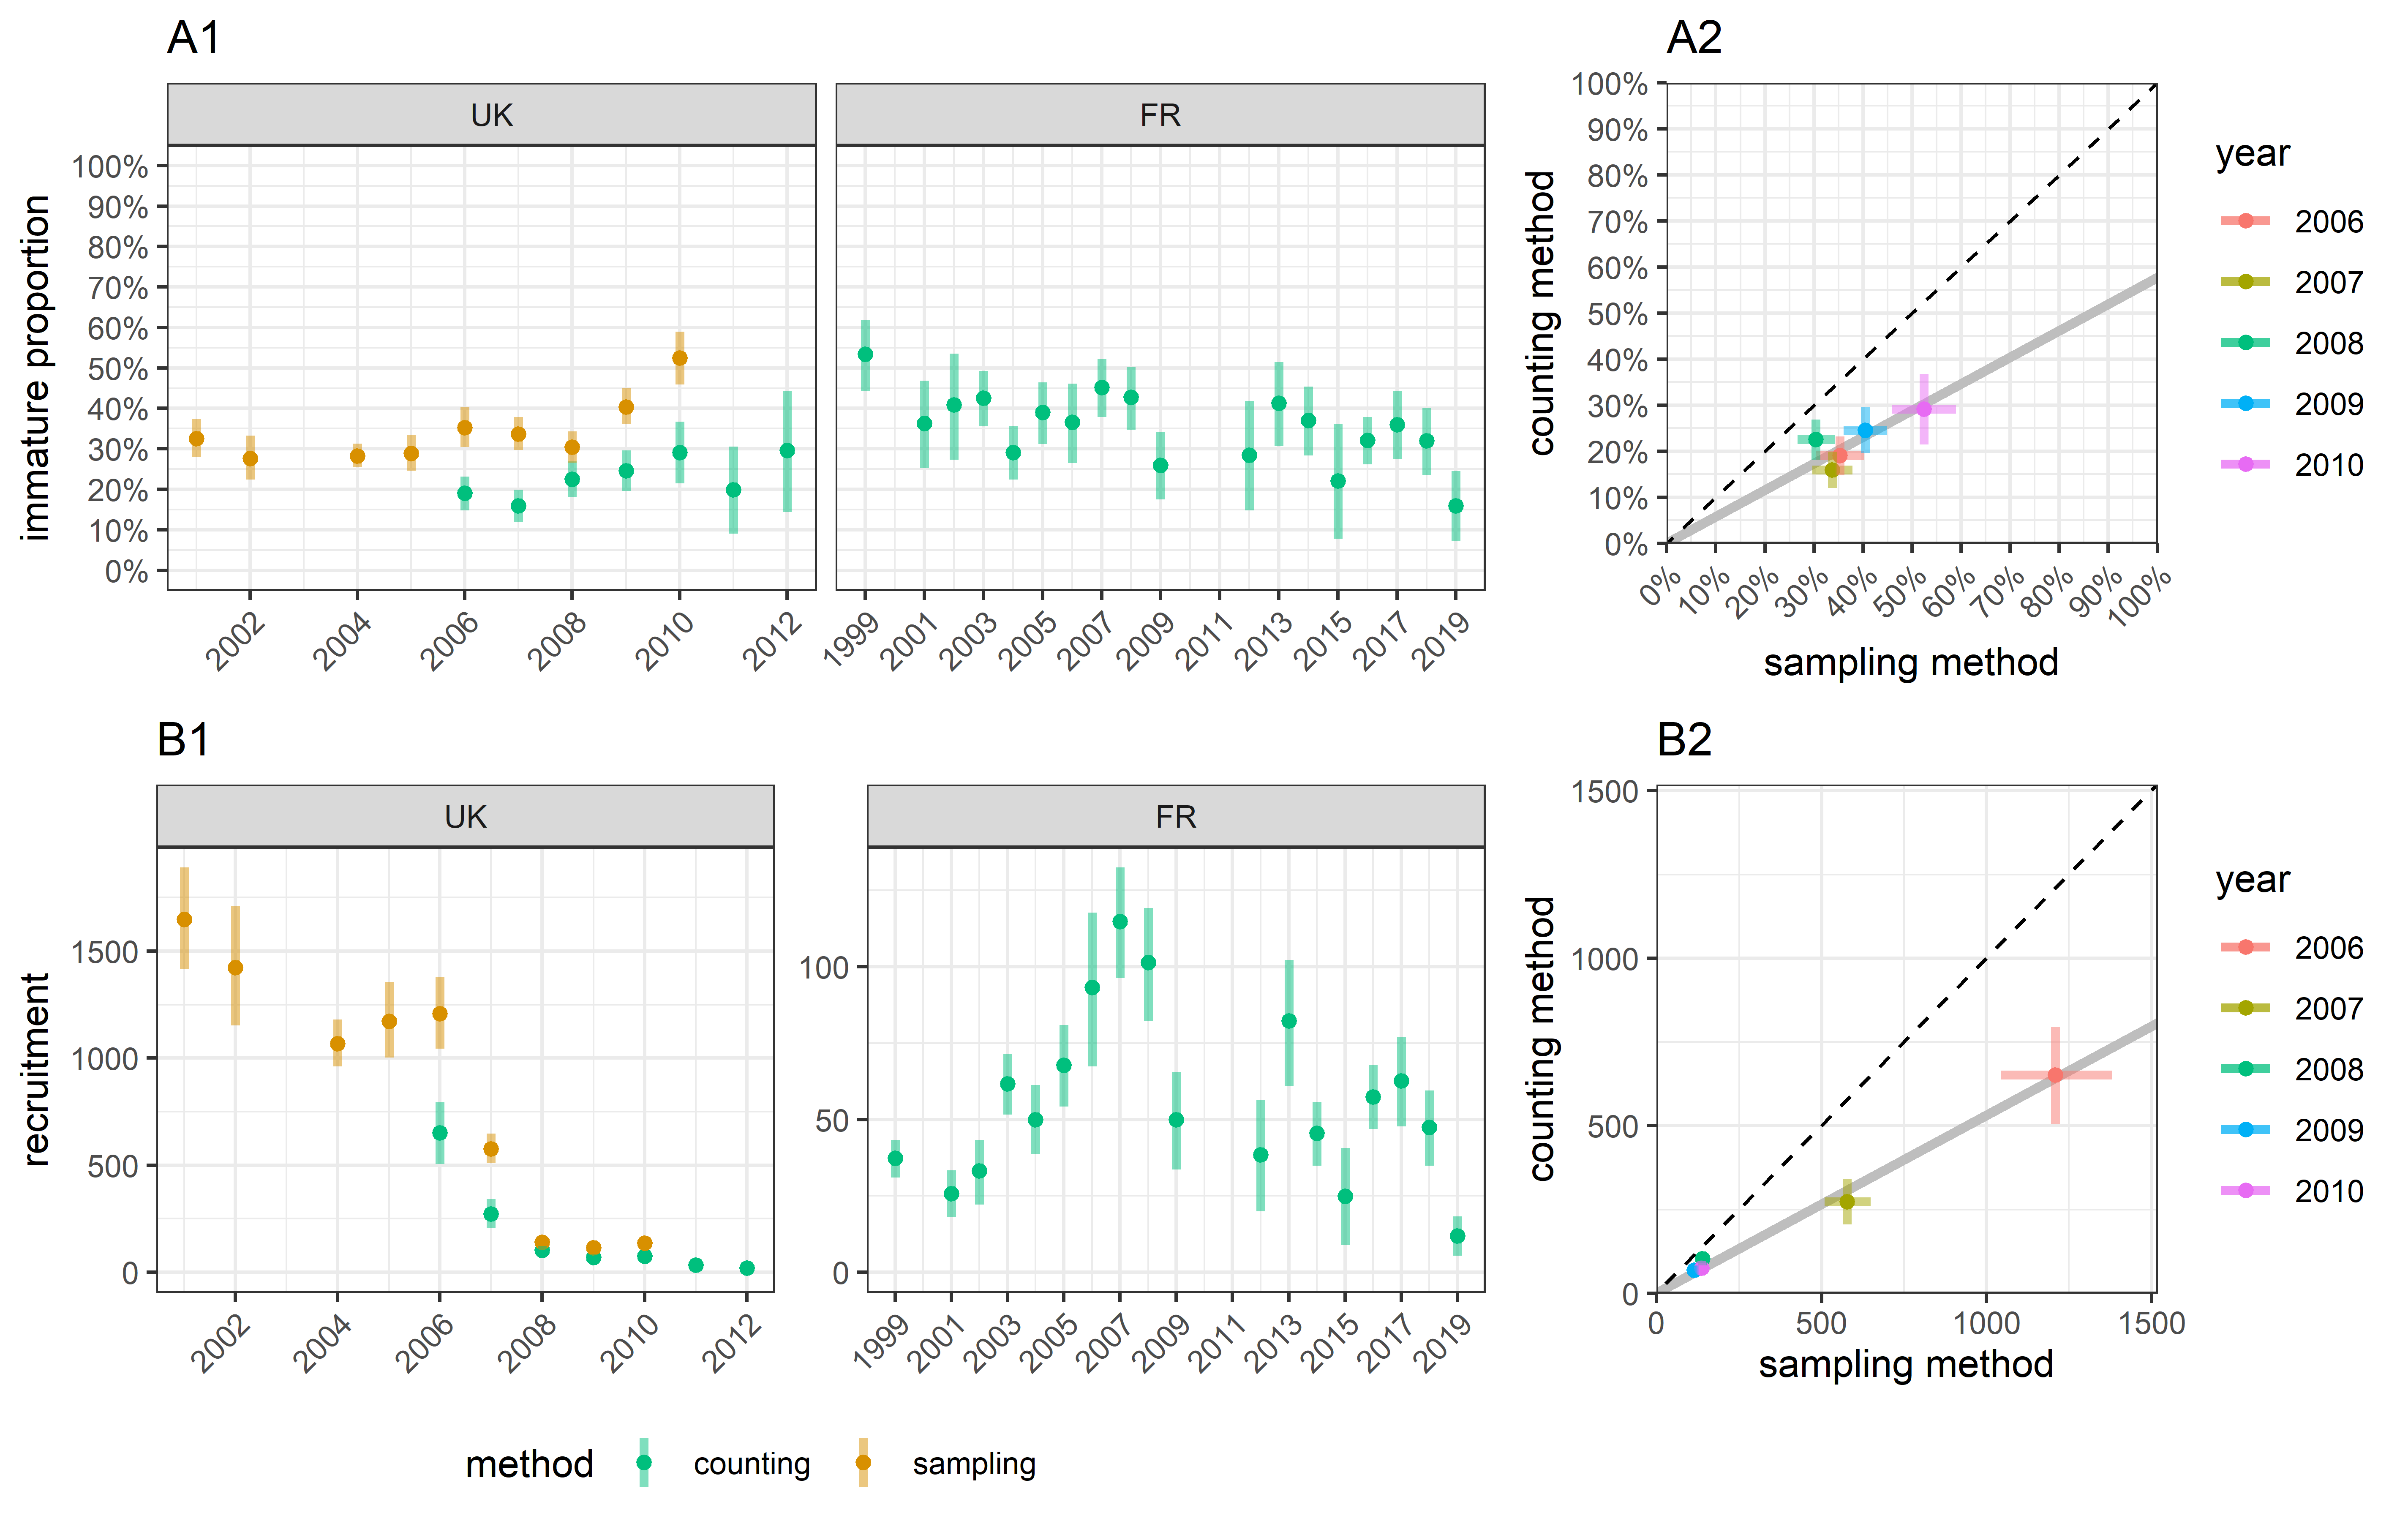
\includegraphics[width=1\linewidth]{../Output/plot_8} 

}

\caption{(A1) Estimates of the proportion of the immature individuals in the wintering population; (B1) estimates of the number of recruits, i.e.~the young adults reproducing for their first time; (A2) \& (B2) comparison of the values between the two estimation methods; bars define the 95\% confidence intervals}\label{fig:sup}
\end{figure}



















\end{document}
